\documentclass{adrian}
\title{\textbf{Sistemas de Telecomunicaciones}}
\author{Adrián Alberdi Ainciburu}
\date{}
\usepackage[top=1in, bottom=1.25in, left=1in, right=1in]{geometry}
%\makeglossaries

\begin{document}
\maketitle
\tableofcontents
%\newglossaryentry{computer}
{
  name=computer,
  description={is a programmable machine that receives input,
               stores and manipulates data, and provides
               output in a useful format}
}
\newacronym[longplural={Kilobits per Second}]{kbps}{kbps}{kilobit per second}	
\section{Introducción}
\subsection{Sistemas de Telecomunicación}
\begin{itemize}
\item\textbf{\Gls{teleco}:} Comunicación (intercambio de información) a distancia.
\item\textbf{\Gls{Sistema}:} Conjunto de medios y de métodos para el logro de un fin común.
\item\textbf{\Gls{Red}:} Conjunto organizado de recursos tanto físicos como lógicos que permiten la telecomunicación. La \gls{Red} es un recurso escaso que debe compartirse. Para esto se aplican técnicas de acceso múltiple y de multiplexación en las redes.
\item\textbf{\Gls{Servicio}:} Conjunto de medios físicos y lógicos operados y gestionados por un proveedor del \gls{Servicio}, que se ponen a disposición de un cliente, junto con unas normas de acceso y utilización, para satisfacer sus necesidades en materia de Telecomunicaciones.
\end{itemize}
\subsubsection{Clasificación de Servicios}
Los servicios se pueden clasificar atendiendo a los siguientes criterios:
\begin{itemize}
\item Básicos y suplementarios: Los servicios básicos son los que existen por sí mismos, como por ejemplo el servicio telefónico básico, en cambio los suplementarios existen asociados a algún servicio básico, como por ejemplo la identificación de llamada.
\item Clasificación \acrshort{ITU}-CCITT: Los servicios portadores son los que transportan la información. Los serviciosfinales o teleservicios incluyen ya el terminal final para poder ofrecer una comunicación completa o añaden capacidades suplementarias como de almacenamiento.
\item Colectivo de usuarios:intercomunicación, comunicación social; comercial, residencial.
\item Capacidad: Banda ancha o estrecha.
\item Modo de efectuar la comunicación: consulta, difusión,conversación, mensajería; simétricos, asimétricos.
\item Movilidad del usuario: movil, portátil, fijo.
\item Tipo de red: \acrshort{RTPC}, \acrshort{RDSI}, Radiodifusión.
\end{itemize}
\subsubsection{Principales servicios}
\begin{itemize}
	\item Servicio Telefónico: Servicio de comunicación por voz entre usuarios. Es un servicio de gran extensión en el cual se han introducido gran cantidad de avances como la digitalización o la movilidad.
	\item Servicio de transmisión de datos: Servicio de intercambio de información de naturaleza digital que se apoya o en la red telefónica o en la red de datos.
	\item Servicios de valor añadido: Servicios como el fax, el teletexto o el datáfono.
	\item Servicios de radiocomunicación: Servicios caracterizados por la inexistencia de un medio físico de enlace, lo que le permite ser movil y dar acceso a grandes públicos.
\end{itemize}
\subsubsection{Arquitectura de un sistema de Telecomunicación}
En la figura a continuación se pueden ver diferentes entidades funcionales y puntos de referencia (interfaces), interconexiones entre entidades funcionales. Las entidades funcionales son el conjunto de funciones en la red con una finalidad común que pueden comprender uno o varios dispositivos físicos, como los terminales, la red de transporte o la terminación de red. Los puntos de referencia (interfaces) son interconexiones entre entidades, en la figura se ven las interfaces U y S.
\begin{figure}[H]
\centering
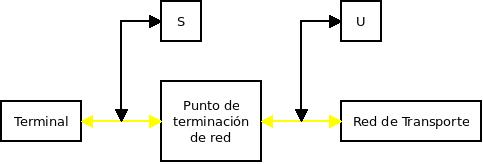
\includegraphics[width=\textwidth]{Imagen/arquisistemateleco.jpg}
\caption{Arquitectura básica de un sistema de Telecomunicación}
\label{}
\end{figure}
\subsection{Organismos reguladores de las Telecomunicaciones}
\begin{itemize}
	\item UIT (\acrshort{ITU}) Unión Internacional de Telecomunicaciones. Tienen la función de armonizar las telecomunicaciones a nivel global y para esto realizan estudios y formulan recomendaciones. Tiene varios organos permanentes
	\begin{itemize}
		\item Secretaría.
		\item UIT-R: Radiocomunicaciones (antiguo CCIR)
		\item UIT-T: Telegrafía, Telefonía y telemática (antiguo CCITT)
		\item Junta de registro de frecuencias
	\end{itemize}
	\item \acrshort{ISO} Organización Internacional de Estandarización. En españa está representada por la Agencia española de Normalización y Certificación. Esta se encarga de la elaboración de normas. Por ejemplo la ISO 9000 se ocupa de la gestión de la calidad.
	\item \acrshort{CEPT} Conferencia Europea de Administraciones de Correos y Telecomunicaciones. Su función es la armonizaciónde las telecomunicaciones a nivel europeo, proporcionando un foro de discusión para el fomento de las relaciones entre organismos reguladores europeos. 
	\item \acrshort{ETSI} European Telecommunication Standards Institute. Fue creado por el CEPT para la elaboración de normas y estandares sobre redes y sistemas.
	\item Dirección General para la Sociedad de la Información de la Comisión Europea. Políticas proyectos y programas relacionados con las tecnologías de la información.
	\item \acrshort{IEEE} Institute of Electrical and Electronic Engineers. Crea normas de efecto global.
	\item \acrshort{WARC} World Administrative Radio Conference. Define que bandas de frecunecia son de uso preferente a servicios concretos (antes eran dedicadas, ahora no).
	\item \acrshort{CNAF} Cuadro Nacional de Atribución de Frecuencias. Es la WARC de españa. Tanto este como el anterior tienen los siguientes roles:
	\begin{itemize}
		\item Atribución (de una banda de frecuencias): inscripción en el cuadro de atribución de bandas de frecuencias, de una banda de frecuencias determinada, para que sea utilizada por uno o varios servicios de radiocomunicación terrenal o espacial o por el servicio de radioastronomía en condiciones específicas. 
		\item Adjudicación (de una frecuencia o de un canal radioeléctrico): inscripción de un canal determinado en un plan, adoptado por una conferencia competente, para ser utilizado por una o varias administraciones para un servicio de radiocomunicación terrenal o espacial en uno o varios países o zonas geográficas determinados y según condiciones específicas.
		\item Asignación (de una frecuencia o de un canal radioeléctrico): autorización que da una administración para que una estación radioeléctrica utilice una frecuencia o un canal radioeléctrico determinado en condiciones específicas. 
	\end{itemize}
\end{itemize}
\subsection{Legislación de Telecomunicaciones}
\subsubsection{Ley 32/2003 de Noviembre}
Deroga la Ley General de Telecomunicaciones 11/1998 de 24 de Abril con el objetivo de liberalizar la competencia en Telecomunicaciones mediante el establecimiento de licencias para prestación de servicios de Telecomunicaciones. También incorpora la evolución de las Telecomunicaciones desde la liberalización, siguiendo las Directivas de la UE.
\subsubsection{Ley 9/2014}
El objetivo es mejorar la libre competencia y facilitar la inversión. Las principales diferencias son la inclusión de medidas estructurales para:
\begin{itemize}
	\item Facilitar el despliegue de nuevas redes (incluyendo expropiación de azoteas)
	\item Mejora de los servicios innovadores para los ciudadanos y abaratamiento de los mismos
\end{itemize}
Además se crea nueva comisión interministerial de \acrshort{RF} y Salud. Se lucha por la simplificación del despliegue de redes (algunas medidas muy controvertidas). Otro objetivo es garantizar que en 2017, el 100\% de los hogares tengan un ancho de banda de 10Mbps y en 2020, a 30MBps (100\%) y más de 100Mbps (50\%).
%% Tema 2
\section{Tema 2}
\subsection{Teoría de colas}
\begin{figure}[H]
\centering
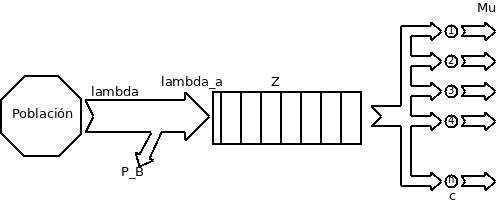
\includegraphics[width=0.9\textwidth]{Imagen/diateocolas.jpg}
\caption{Diagrama teoría de colas}
\label{dia:teocolas}
\end{figure}

\begin{itemize}
	\item $\mu$: Tasa de servicio, velocidad del sistema. Se mide en usuarios por unidad de tiempo.\\
	\item $\lambda$: Tasa de llegadas. Se mide en usuarios por unidad de tiempo.\\
	\item $\lambda_a$:Tasa de llegadas efectiva, la anterior menos los usarios expulsados del sistema. Se mide en usuarios por unidad de tiempo.\\
	\item c: Número de servidores del sistema.\\
	\item Z: Sistema de cola, lo más común FIFO.\\
\end{itemize}
Para analizar el sistema siempre hay que asumir dos cosas: que el sistema no está colapsado y que se está produciendo un reparto uniforme entre todos los servidores.\\
\begin{equation}%[Tráfico ofrecido]
A_o=\frac{E(s)}{E(r)}=\frac{\lambda}{\mu}\text{ E=Tiempo/Tiempo}
\end{equation}
\begin{equation}%[Tráfico cursado]
A_c=A_0(1-P_B)=\frac{\lambda_a}{\mu}\text{ E=Tiempo/Tiempo}
\end{equation}
\begin{equation}%[factor de utilización]
\rho=\frac{A_c}{c}=\frac{\lambda_a}{\mu C}\text{ adimensional}
\end{equation}
\begin{example}
1 petición/hora se resuelve a 1 minuto/petición con una probabilidad de bloqueo 0. Calcula el factor de utilización para 1, 2 y 3 servidores:\\
\[A_o=A_c\]
\[A_o=\frac{\lambda}{\mu}=1\sfrac{pet}{h}1\sfrac{min}{pet}\sfrac{1h}{60min}=\sfrac{1}{60}E=16.7mE\]\\
\[\rho=\frac{A_c}{c}=
\begin{cases}
\sfrac{16.7}{1}=1.67\% & \text{para } c=1\\
\sfrac{16.7}{2}=0.83\% & \text{para } c=2\\
\sfrac{16.7}{3}=0.56\% & \text{para } c=3
\end{cases}\]
\end{example}

\subsubsection{Fórmulas de Little}
Las fórmulas de little son el resultado del análisis de las colas en régimen permanente.
\begin{itemize}
	\item $N(t)$: Número de usuarios en el sistema en un tiempo t.
	\item $N_s(t)$: Número de usuarios en los servidores en un tiempo t.
	\item $N_q(t)$: Número de usuarios en la cola en un tiempo t.
\end{itemize}
\begin{align}%[Fórmulas de little]
N=N_s+N_q\to L &=L_s+L_q\to W=W_s+W_q\\
L_x &=\gamma W_x\\
W_s=E(s)=\sfrac{1}{\mu} & \Leftrightarrow L_s=A_c\\
\gamma &=\lambda_a
\end{align}
\subsubsection{Distribución exponencial}
\begin{figure}[H]
\centering
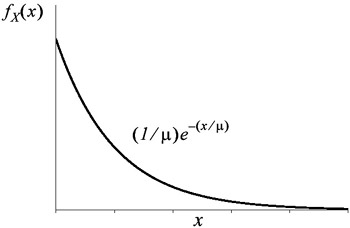
\includegraphics[width=0.9\textwidth]{Imagen/distribucionexponencial.jpg}
\caption{Distribución Exponencial}
\end{figure}
\begin{align}
P(t)=\mu e^{-\mu t} \leftarrow t\geq 0\\
Media=E(s)=\sfrac{1}{\mu}\\
P(t\leq T)=1-e^{-\mu T}
\end{align}
\subsubsection{Distribución de Poisson}
%%Insertar foto de la distribución de Poisson
\begin{figure}[H]
\centering
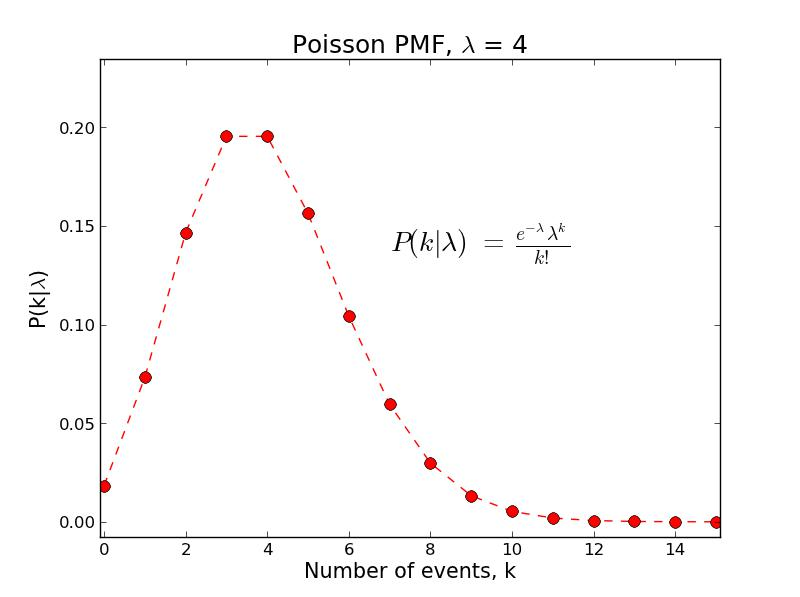
\includegraphics[width=0.9\textwidth]{Imagen/distribucionpoisson.jpg}
\caption{Distribución de Poisson}
\label{}
\end{figure}
\begin{equation}
P(k)=\frac{Ke^{-k}}{K!}
\end{equation}
\subsubsection{Nomenclatura teoría de colas}
\begin{center}
\framebox[1.1\width]{\huge{A/B/c/k/m/Z}} \par
\end{center}
\begin{itemize}
\item {A:} tiempo entre llegadas. m es la distribución normal(Poissoniana), i un modelo determinista y gi es el modelo general.
\item {B:} tasa de servicio. m es la distribución normal(Exponencial), i un modelo determinista y gi es el modelo general.
\item {c:} número de servidores.
\item {k:} capacidad del sistema. En caso de no venir especificado se asume capacidad "infinita".
\item {m:} tamaño de la población. En caso de no venir especificado se asume población "infinita".
\item {Z:} disciplina de la cola. En caso de no venir especificado se asume una cola FIFO.
\end{itemize}
Cuando se habla de poblaciones o capacidades infinitas en realidad significa que el número es mucho mayor que el número de servidores. Población/Capacidad>>c.
\subsubsection{Modelo M/M/1}
Un modelo con llegadas poissonianas, tasa de servicio exponencial, 1 único servidor, una cola infinita, población infinita y una cola con disciplina FIFO. Este modelo tiene una probabilidad de bloqueo nula $P_B=0$ con lo cual se cumple lo siguiente: $A_c=A_o=\sfrac{\lambda}{\mu}$. Al tener un solo servidor además se ve que $\rho=A_o$.
\begin{example}[M/M/1]
Tasa de llegadas 30$\sfrac{\text{clientes}}{\text{hora}}$ con una tasa de servicio de 115$\sfrac{\text{segundos}}{\text{cliente}}$ en un único servidor.
\[A_c=A_o=\frac{\lambda}{\mu}=30*115\sfrac{1}{3600}=0.9583E\] \\
\[\rho=A_c=A_0=0.9583=95.83\%\] Como se puede ver el servidor está a punto de saturarse.\\
\[L=\frac{\rho}{1-\rho}=23\text{ usuarios en el sistema de media}\]
\[L=\frac{\rho^2}{1-\rho}=22\text{ usuarios en la cola de media}\]
\[W=\frac{E(s)}{1-\rho}=45.96\text{ minutos en el sistema de media}\]
\[W=\frac{\rho E(s)}{1-\rho}=44.06\text{ minutos en la cola de media}\]
Los usuarios se quejarán. Hay que esperar 44 minutos en la cola para un servicio que tarda 2 en ser servido.
\end{example}
\subsubsection{Modelo M/M/c}
Un modelo con llegadas poissonianas, tasa de servicio exponencial, c servidores idénticos, una cola infinita, población infinita y una cola con disciplina FIFO. Este modelo tiene una probabilidad de bloqueo nula $P_B=0$ con lo cual se cumple lo siguiente: $A_c=A_o=\sfrac{\lambda}{\mu}$.\\
\begin{example}[M/M/c]
Continuando el ejemplo anterior. $\lambda=30\sfrac{\text{clientes}}{\text{hora}}$ con una media de tiempo de servicio $\text{E(s)}=\sfrac{1}{\mu}=115\sfrac{\text{segundos}}{\text{cliente}}$. Contamos con 2 sevidores en lugar de uno. Compararlo con el anterior: W=46min $\text{W}_{\text{q}}$=44min\\
\begin{gather*}
A_o=\frac{\lambda}{\mu}=0.9583E=A_c\\
\rho=\frac{A_c}{c}=0.47915\simeq 48\% \\
L_q=\frac{\rho C(A_o,c)}{(1-\rho)}=0.28\text{ clientes en la cola de media}\\
W_q=\frac{E(s)C(A_o,c)}{c(1-\rho)}=34.2\text{ segundos en la cola de media}
\end{gather*}
Se puede ver una gran mejoría entre los 44 minutos con un único servidor y los 34 segundos en el caso de dos servidores.
\end{example}
\subsubsection{Modelo M/M/c/c}
Un modelo con llegadas poissonianas, tasa de servicio exponencial, c servidores idénticos, sin colas, población infinita y una cola con disciplina FIFO. En este modelo es en el primero que vemos una probabilidad de bloqueo distinta de cero, $P_B=B(A_o,c)$ esta probabilidad se puede calcular gráficamente con las gráficas del Erlang B. En cambio aplicando esto a las fórmulas de little podemos ver lo siguiente: $L_q=0\to L=L_s=A_c=A_o(1-P_B)$\\
\begin{example}[M/M/c/c]
8 servidores con $E(s)=\sfrac{1}{\mu}=4\sfrac{\text{h}}{\text{usuario}}$ y una tasa de llegadas $\lambda=3\sfrac{\text{usuarios}}{\text{h}}$\\
\begin{gather*}
A_o=\frac{\lambda}{\mu}=12E\\
P_B=B(12,8)=42\%
\end{gather*}
\end{example}
\subsection{Estructura de la red telefónica}
Se trata de un sistema con bloqueo, se puede variar con sistemas adicionales como el buzón de voz o similares a un sistema con espera. Cuando era analógica la red telefónica se trataba de un sistema de conmutación de circuitos.\\
Las centrales de conmutaciónse basan en la idea de conmutación multietapa, con esto se evita el tener un cable por destino. La estructura jerarquica de la red telefónica está descrita a continuación:
\begin{itemize}
\item Un par de abonado entre cada cliente y la central local. [CL]
\item Central primaria enlaza 2 o más centrales locales. [CP]
\item Bucle de abonado, del abonado a la central local.
\item Enlace troncal, los internos entre centrales, también llamados enlace final.
\item Central secundaria une dos o más centrales primarias. [CS]
\item Central terciaria y superiores enlazan dos o ás centrales de orden inferior. [CT]
\item Una ruta final está unicamente formada por enlaces finales.
\end{itemize}
\begin{figure}[H]
\centering
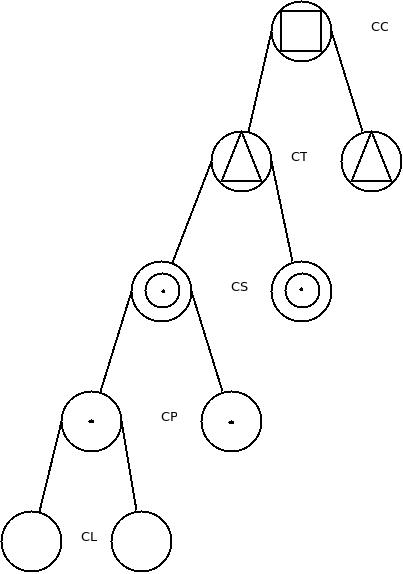
\includegraphics[width=0.9\textwidth]{Imagen/diajerartelefono.jpg}
\caption{Diagrama de la red jerárquica}
\label{diaRedTelefonica}
\end{figure}
A parte de la red jerarquica existe la red complementaria. Esta está formada por enlaces directos. Enlaces que unen centrales que no están unidas jerarquicamente.\\
\subsubsection{Encaminamiento en la estructura de la red telefónica}
\begin{enumerate}
\item Identificamos el arbol de destino. Está formado por todos los nodos jerarquicamente superiores al nodo de destino.
\item En cada nodo vemos si hay una sección directa que nos lleve al arbol de destino. No se pueden tomar 2 secciones directas en la misma ruta. Una sección directa nunca desbordará sobre otra sección directa, siempre desbordará sobre la sección final.
\item una vez en el arbol de destino desciendo jerarquicamente hasta el nodo destino.
\end{enumerate}
\begin{example}[Encaminamiento en la red telefónica]
\begin{figure}[H]
\centering
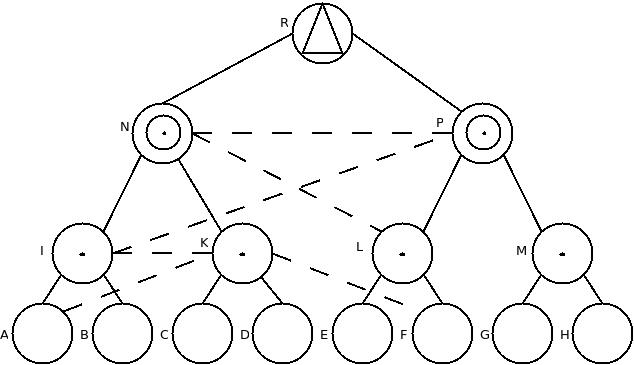
\includegraphics[width=0.9\textwidth]{Imagen/ejemploredtelefonica.jpg}
\label{}
\end{figure}
De la figura podemos sacar las siguientes rutas.\\
\begin{center}
\begin{tabular}{c c c c}
A$\to$C & AKC  		& A$\to$E 	& AIPLE 	\\
 		& AIKC 		&			& AINLE		\\
 		& AINKC		&			& AINRPLE	\\
E$\to$A & ELNIA  	& 		 	& 		 	\\
 		& ELPIA 	&			& 			\\
 		& ELPRNIA	&			& 			\\
\end{tabular}
\end{center}
Como se puede ver no todas las rutas son 100\% simétricas.
\end{example}
\subsubsection{Red inteligente}
Surge con la digitalización y a la vez que la Red Digital de Servicios Integrados (RDSI). Este sistema ofrece servicios de valor añadido.
\begin{figure}[H]
\centering
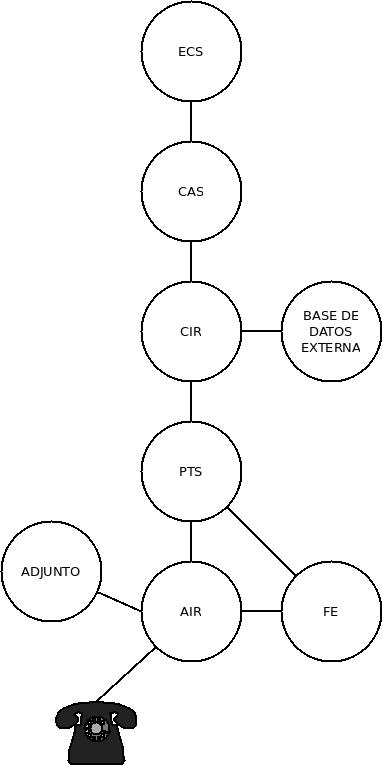
\includegraphics[width=0.5\textwidth]{Imagen/diaredinteligente.jpg}
\caption{Diagrama de la Red Inteligente}
\end{figure}
\begin{itemize}
\item Agencia de Inteligencia de Red [AIR]: Identifica si la llamada está destinada a la Red Inteligente. Solo hay una por Central Local.
\item Punto de Transferencia de Señalización [PTS]: Es un centro de intercambio entre las diferentes partes de la red.
\item Centro de Inteligencia de Red [CIR]: Es la parte más importante de la Red Inteligente ya que es el que reconoce los servicios y da las ordenes.
\item Adjunto: Es como el CIR pero se encuentra en la Central Local. De esta forma descarga las instancias superiores de la red.
\item Módulo de Funciones Especiales [FE]: Cumple varias funciones como la sintesis de voz o la captación de teclas marcadas.
\item Base de datos externa: Se trata de un conjunto de bases de datos que no se encuentran dentro del CIR, como la de tarjetas de crédito.
\item Centro de Administración de Servicios [CAS]: Lugar donde se administra y controla todos los servicios de la red. Este no tiene por que estar conectado a la red constantemente.
\item Entorno de Creación de Servicios [ECS]: Lugar donde se implementan los nuevos servicios. Este no tiene por que estar conectado a la red constantemente.
\end{itemize}
\subsubsection{Ejercicios}
\begin{exercise}[5]
La red telefónica de la figura tiene una probabilidad de pérdidas en las secciones finales del 1\% y una probabilidad de desbordamiento en las secciones directas del 10\% .
\begin{figure}[H]
\centering
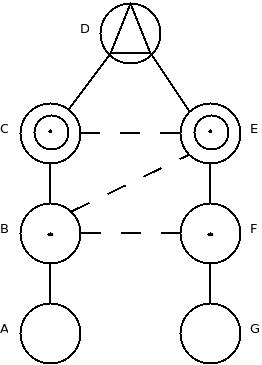
\includegraphics[width=0.5\textwidth]{Imagen/ejercicio5tema1.jpg}
\label{}
\end{figure}
La matriz de tráfico (simétrica) en Erlangs es la siguiente:
\begin{center}
\begin{tabular}{| c | c | c | c | c | c | c | c |}
\hline
   & A & B & C & D & E & F & G \\\hline
 A & - & 10 & 15 & 5 & 2 & 1 & 1 \\\hline
 B &   & - & 50 & 15 & 6 & 3 & 2 \\\hline
 C &   &   & - & 80 & 30 & 10 & 5 \\\hline
 D &   &   &   & - & 90 & 15 & 5 \\\hline
 E &   &   &   &   & - & 60 & 18 \\\hline
 F &   &   &   &   &   & - & 12 \\\hline
\end{tabular}
\end{center}
Se pide:\\
\textbf{1.} Indicar los caminos que comunican los nodos E y A.\\
\begin{center}
\begin{tabular}{c c c c}
E$\to$A & EBA  		& A$\to$E 	& ABE 	\\
 		& EDCBA		&			& ABCE	\\
 		& 			&			& ABCDE	\\
\end{tabular}
\end{center}
\textbf{2.} Calcular el tráfico ofrecido y cursado en la sección directa C$\to$E.\\
\begin{gather*}
TO_{C\to E}=TO_{CEpropio}+TO_{BEdesb}+TO_{BFdesb}+TO_{CF}+TO_{CG}=\\
30+0.8+0.7+10+5=46.5E\\
TO_{BE}=TO_{BEpropio}+TO_{AE}=8E\\
TO_{BEdesb}=TO_{BE}P_d=TO_{BE}0.1=0.8E\\
TO_{BF}=TO_{BFpropio}+TO_{BG}+TO_{AF}+TO_{AG}=7E\\
TO_{BFdesb}=TO_{BF}P_d=TO_{BF}0.1=0.7E\\
TC_{C\to E}=TO_{C\to E}(1-P_D)=41.85E
\end{gather*}
\textbf{3.} Considerando solo el tráfico saliente de A y sabiendo que la probabilidad de que la duración de la llamada sea superior a 5 minutos es de 0.08205, ¿cuál es la duración media de la llamada?\\
Se trata de un sistema con bloqueo M/M/c/c con $A_{oA}=34E=\frac{\lambda}{\mu}$.
\begin{gather*}
P(W>5min)=\int_{5}^{\infty}\mu e^{-\mu t}dt=-e^{-\mu t}\Big|_{5}^{\infty}=0.08205\\
\mu=0.5\sfrac{llamadas}{minuto}\to E(s)=2\sfrac{minutos}{llamada}
\end{gather*}
\textbf{4.} ¿Cuántos intentos de llamada se hacen en la hora cargada(HC)?\\
\begin{gather*}
A_{oA}=34E=\frac{\lambda}{\mu}\\
\mu=0.5\sfrac{llamadas}{minuto}\\
\lambda=34*0.5=17\sfrac{llamadas}{minuto}\\
\lambda_{HC}=17*60=1020\sfrac{llamadas}{hora}
\end{gather*}
\textbf{5.} Los registradores de la central A analizan las primeras cifras y encaminan las llamadas, pudiéndose modelar como un sistema M/M/c. Si el tiempo de ocupación de los registradores por cada llamada es de 6 segundos, ¿cuántos son necesarios para que la probabilidad de esperar más de 1 segundo sea de 0.008?\\
\begin{gather*}
E(s')=6\sfrac{segundos}{llamada}\to A'_o=\frac{\lambda}{\mu '}=1.7E\\
P(W_q>1s)=0.008=C(c,A'_o)e^-c\mu 'T(1-\rho)
\end{gather*}
Este apartado habrá que hacerlo por prueba y error hasta hallar el número de servidores necesarios para cumplir con las especificaciones. Se puede ver estas pruebas en la tabla:\\
\begin{center}
\begin{tabular}{c | c | c | c}
$C(c,A'_o)$ & c & $\rho$ & $P(W_q>1)$ \\\hline
0.7  & 2 & 0.85  & 0.6672 \\
0.1  & 4 & 0.425 & 0.0692 \\
0.008 & 6 & 0.283 & 0.00402
\end{tabular}
\end{center} 
De la tabla se puede observar que el número mínimo de registradores ha de ser 6.\\
\textbf{6.} ¿Cuál es el tiempo medio de espera en los registradores?\\
\[W_q=\frac{E(s)\rho}{1-\rho}=2.3682segundos\]
\end{exercise}
\begin{exercise}[6]
En un territorio de un país en vías de desarrollo, se ha decidido crear una nueva red telefónica digital. Para su planificación se han considerado los siguientes datos:
\begin{itemize}
\item Tras agrupar geográficamente los diferentes núcleos en entidades de población, resultando 83, se han obtenido 70 entidades  con 20000 habitantes, 10 con 60000, 2 con 1000000 y 1 (la capital) con 2000000
\item Se considera un grado inicial de penetración del servicio del 30\% (30 teléfonos por cada 100 habitantes). El incremento futuro de dicho porcentaje será absorbido por las correspondientes ampliaciones.
\item El tráfico total (entrante y saliente, excluyendo el local) por abonado se cifra en 20mE.
\item Se dispone de unidades locales de 6000 líneas.
\item Las centrales primarias tienen una capacidad para 3000E de tráfico total (entrante y saliente).
\item Existirá una central secundaria por cada 5 primarias y solo una central terciaria.
\item Sólo se establecen rutas finales, con una probabilidad de pérdida del 2\% (se puede aproximar la función de Erlang B por $B(A_o,c)=0.025\sfrac{A_o}{c}$.
\end{itemize}
Se desea conocer:\\
\textbf{1.} El número de unidades locales de conmutación necesarias.\\
\begin{gather*}
CL=(70\frac{20000}{6000}+10\frac{60000}{6000}+2\frac{1000000}{6000}+1\frac{2000000}{6000})30\%\\
CL=300\text{ centrales locales}
\end{gather*}
\textbf{2.} Los sistemas MIC de norma europea que permitirán la conexión de cada unidad local con su correspondiente primaria.\\
Cada unidad local genera $A_{oCL}=6000*0.02=120E$ con una probabilidad de pérdida del 2\% y utilizando la función Erlang B obtenemos:
\begin{gather*}
B(A_o,c)=0.025\sfrac{A_{oCL}}{c}=0.02\\
c=\frac{0.025A_{oCL}}{0.02}=150\text{ canales}\\
MIC=\frac{c}{30}=5\text{ sistemas MIC de norma europea}
\end{gather*}
\textbf{3.} El número de centrales primarias.\\
\[CP=\frac{300}{\frac{3000E}{6000*0.02E}}=12\text{ centrales primarias}\]
\textbf{4.} El número de centrales secundarias.\\
\[CS=\frac{12}{5}=2.4\to 3\text{ centrales secundarias}\]
\end{exercise}
\begin{exercise}[7]
Con motivo del cambio de numeración de 6/7 cifras a 8 se contempla la digitalización de la red telefónica de un país. Para ello, se realiza el diseño de la red basándose en los siguientes datos:
\begin{itemize}
\item La capacidad de las unidades locales (centrales urbanas) es de 40000 líneas.
\item La capacidad de las centrales de tránsito (primarias y secundarias) es de 40000 enlaces.
\item Las centrales locales de cada núcleo urbano se conectarán mediante secciones directas en malla (todas con todas) para cursar, en primera instancia el tráfico urbano.
\item Las centrales locales se conectarán a una de las centrales secundarias (ruta directa) para cursar, como primera alternativa, el tráfico interurbano y el internacional.
\item Cada central local se conectará a su correspondiente central primaria (ruta final), para el desbordamiento del tráfico anterior.
\item Cada central primaria se conectará a su secundaria jerárquica ( ruta final), constituyendo éstas entre si una red mallada.
\item Considerando despreciable la pérdida de tráfico originada por saturación de las diferentes centrales, se prevén, para los enlaces y correspondientes medios de transmisión unas probabilidades del 1\% de pérdidas y del 10\% de desbordamiento.
\item Se estima un tráfico por abonado de 100mE, desglosado del siguiente modo:
\subitem 10+0.015A mE para tráfico urbano, al 50\% entre entrante y saliente, siendo A el número de abonados del núcleo urbano en miles.
\subitem Resto para tráfico interurbano e internacional, que se distribuye al 50\% entre entrante y saliente.
\end{itemize}
OBSERVACIONES:
\begin{itemize}
\item Se considera despreciable el tráfico local (entre abonados de la misma central local).
\item Se puede aproximar la distribución Erlang-B por la expresión $B(c,A_o)=8.33*10^{-3}\sfrac{c}{A_o}$ para el 1\% y $B(c,A_o)=0.1\sfrac{c}{A_o}$ para el 10\%.
\item Considerar que las centrales de tránsito por cada llamada son necesarios dos enlaces, uno de entrada y otro de salida.
\end{itemize}
\textbf{1.} Eficiencia (E/enlace) de las rutas directas y finales.\\
\begin{gather*}
B(c,A_o)=8.33*10^{-3}\frac{c}{A_o}\sfrac{enlace}{E}=1\% \to 8.33*10^{-3}\frac{1}{\eta_{RF}}=1\% \\
\eta_{RF}=8.33*10^{-3}\frac{1}{1\%}=0.833\sfrac{E}{enlace}\\
B(c,A_o)=0.1\frac{c}{A_o}\sfrac{enlace}{E}=10\% \to 0.1\frac{1}{\eta_{RF}}=10\% \\
\eta_{RF}=0.1\frac{1}{10\%}=1\sfrac{E}{enlace}
\end{gather*}
\textbf{2.} Capacidad de tráfico (E)de las centrales primarias.\\
\begin{gather*}
C_CP=\frac{40000}{2}\eta_{RF}=16660E
\end{gather*}
\textbf{3.} Distribución, en las cenrales secundarias, entre enlaces de secciones directas y finales, y la capacidad de tráfico de dichas centrales.\\
\begin{gather*}
\begin{cases}
N_{RD}+N_{RF}=\frac{40000}{2}\\
N_{RD}\eta_{RD}=N_{RF}\eta_{RF}
\end{cases}
N_{RD}=17547enlaces\\
N_{RF}=2453enlaces\\
C_{CS}=N_{RD}\eta_{RD}+N_{RF}\eta_{RF}=19590E
\end{gather*}
\textbf{4.} Considerando una capacidad de 16000E y 19600E para las centrales primarias y secundarias, respectivamente, evaluar, para un núcleo de 3.5 millones de abonados, el número de centrales locales, primarias y secundarias necesario.\\
Asumiendo $C_{CP}=16000E$ y $C_{CS}=19600E$ y una población $A=3.5*10^6abonados$
\begin{gather*}
N_{CL}=\frac{A}{40000}=87.5\to88\text{ centrales locales}\\
N_{CP}=10\% a_o
\end{gather*}
\textbf{5.} Si se reserva el prefijo 0 para servicios especiales y el prefijo 9 para el acceso interurbano, estimar la capacidad (número máximo de abonados que admite) del nuevo plan de numeración. Considerar que si el número local es del tipo ZXXXXXXX, el número nacional de 10 dígitos se formará anteponiendo el prefijo 0X.\\
hola
\end{exercise}
\begin{exercise}[8]
En el servicio de cobro revertido automático (SCRA), también llamado "Línea 900", el cobro de la llamada se carga, de manera automática, al abonado llamado, y no al llamante. Un nuevo operador de telecomunicaciones pretende ofertar dicho servicio mediante la estructura de red de la figura.\\
%%Incluir imagen
\myworries{Incluir imagen del ejercicio}
El servicio funciona de la siguiente forma: cuando un usuario marca un número 900.XXX.XXX, se encamina la llamada a una central específica, que realiza la traducción de dicho número y transfiere la comunicación a este último número, al cual le carfa el coste de la llamada. En la planificación del servicio, se han tenido en cuenta las siguientes estimaciones de tráfico:
\begin{itemize}
\item Desde Madrid se originarán, en la Hora Cargada (HC) y para la SCRA, 12000 llamadas, de las que el 0.127\% superarán los 10 minutos.
\item El tráfico total dirigido al SCRA de toda España será 4 veces el originado en Madrid.
\item Para todas las rutas, la probabilidad de pérdida es del 1\%
\end{itemize}
OBSERVACIÓN: Puede aproximar la distribución Erlang-B por la expresión $B(c,A_o)=8.2*10^{-3}\sfrac{c}{A_o}$\\
NOTA: Una empresa puede tener múltiples núeros del tipo 9XX.XXX.XXX (por ejemplo, uno por provincia donde tenga una oficina( y tener, en cambio un único 900.XXX.XXX; al traducir este último, se optará por alguno de los anteriores en base a criterios preestablecidos (por ejemplo, el origen de la llamada).\\
Se desea:\\
\textbf{1.} Dibuje la arquitectura de la Red Inteligente que soporta dicho servicio, indicando claramente qué entidades funcionales aparecen y cuáles se corresponden con el dibujo de la figura.\\

\textbf{2.} Para la ruta de la provincia de Madrid: tráfico (en Erlangs), número de canales (o circuitos), número de sistemas MIC de norma europea.\\

\textbf{3.} Para cada una de las rutas de entrada en RTB: tráfico (en Erlangs), número de canales (o circuitos), número de sistemas de 8 MBps (E2 de 120 canales).\\
\end{exercise}
\begin{exercise}[9]
En la red telefónica de la figura se muestran las rutas finales y las secciones directas. La probabilidad de bloqueo es del 1\% y una probabilidad de desbordamiento del 10\% . Sobre esta red, se le pide lo siguiente:
\begin{figure}[H]
\centering
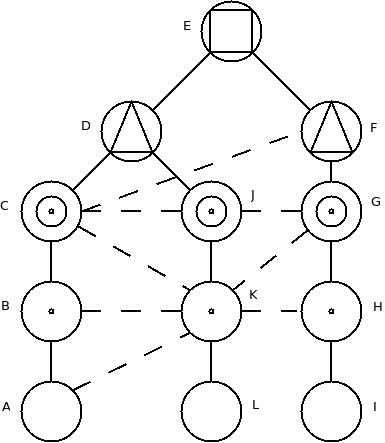
\includegraphics[width=0.5\textwidth]{Imagen/ejercicio9tema1.jpg}
\label{}
\end{figure}
\textbf{1.} Indique las rutas entre las siguientes centrales:\\
\begin{center}
\begin{tabular}{c c c c}
A$\to$L & AKL  		& L$\to$A 	& LKA 	\\
 		& ABKL		&			& LKJCBA	\\
 		& ABCKL		&			& LKJDCBA	\\
 		& ABCDJKL	&			& 	\\
A$\to$I & ABCFGHI  	& L$\to$I 	& LKHI 	\\
 		& ABCDEFGHI	&			& LKJGHI	\\
 		& 			&			& LKJDEFGHI	\\
I$\to$L & IHKL  	& 		 	&  	\\
 		& IHGKL		&			& 	\\
 		& IHGFEDJKL	&			& 	\\
\end{tabular}
\end{center}
\textbf{2.} Calcule el tráfico ofrecido y el tráfico cursado en la sección directa JC/CJ y en la sección final CD/DC.\\
\begin{center}
\begin{tabular}{| c | c | c | c | c | c | c | c | c | c | c | c | c |}
\hline
   & A & B  & C  & D  & E  & F  & G & H  & I  & J  & K  & L \\\hline
 A & - & 15 & 15 & 10 & 5  & 5  & 5 & 10 & 2  & 1  & 8  & 2 \\\hline
 B &   & -  & 15 & 10 & 4  & 5  & 5 & 10 & 2  & 1  & 9  & 1 \\\hline
 C &   &    & -  & 10 & 10 & 20 & 5 & 10 & 5  & 1  & 5  & 5 \\\hline
 D &   &    &    & -  & 10 & 10 & 5 & 1  & 1  & 1  & 0  & 1 \\\hline
 E &   &    &    &    & -  & 5  & 5 & 25 & 10 & 5  & 1  & 0 \\\hline
 F &   &    &    &    &    & -  & 5 & 5  & 10 & 5  & 1  & 1 \\\hline
 G &   &    &    &    &    &    & - & 10 & 5  & 10 & 5  & 5 \\\hline
 H &   &    &    &    &    &    &   & -  & 10 & 15 & 5  & 5 \\\hline
 I &   &    &    &    &    &    &   &    & -  & 10 & 5  & 5 \\\hline
 J &   &    &    &    &    &    &   &    &    & -  & 10 & 10 \\\hline
 K &   &    &    &    &    &    &   &    &    &    & -  & 10 \\\hline
\end{tabular}
\end{center}
Empezamos por calcular el tráfico ofrecido en un sentido y luego en el otro.
\begin{gather*}
TO_{CJ}=TO_{CJpropio}+TO_{AJ}+TO_{BJ}=3E\\
TO_{JC}=TO_{JCpropio}+TO_{KCdesb}+TO_{KBdesb}+TO_{KAdesb}+TO_{JA}+TO_{JB}\\
TO_{KC}=TO_{KCpropio}+TO_{LC}=10\\
TO_{KB}=TO_{KBpropio}+TO_{LB}=10\\
TO_{KA}=TO_{KApropio}+TO_{LA}=10\\
TO_{JC}=1+1+1+1+1+1=6\\
TO_{CD}=TO_{CDpropio}+TO_{CFdesb}+TO_{CJdesb}+TO_{CKdesb}+TO_{CE}+TO_{AD}+TO_{AE}+TO_{BD}+TO_{BE}\\
TO_{CF}=TO_{CFpropio}+TO_{CG}+TO_{CH}+TO_{CI}+TO_{BF}+TO_{BG}+TO_{BH}+TO_{BI}+TO_{AF}+TO_{AG}+\\
+TO_{AH}+TO_{AI}=84E\\
TO_{CJ}=3E\\
TO_{CK}=TO_{CKpropio}+TO_{BKdesb}+TO_{CL}\\
TO_{BK}=TO_{BKpropio}+TO_{AKdesb}+TO_{BL}\\
TO_{AK}=TO_{AKpropio}+TO_{AL}=10E\\
TO_{BK}=11E\\
TO_{CK}=11.1E\\
TO_{CD}=10+8.4+0.3+1.11+10+10+5+10+4=58.81E\\
TO_{DC}=TO_{DCpropio}+TO_{FCdesb}+TO_{JCdesb}+TO_{EC}+TO_{DB}+TO_{EB}+TO_{DA}+TO_{EA}\\
TO_{FC}=TO_{FCpropio}+TO_{GC}+TO_{HC}+TO_{IC}+TO_{FB}+TO_{GB}+TO_{HB}+TO_{IB}+TO_{FA}+TO_{GA}+\\
+TO_{HA}+TO_{IA}=84E\\
TO_{JC}=6E\\
TO_{DC}=10+8.4+0.6+10+10+5+10+4=58E
\end{gather*}
Para terminar calcularemos el tráfico cursado en cada uno de los tramos como $TC=TO(1-P_B)$ siendo $P_B$ la probabilidad de bloqueo en las rutas finales y la probabilidad de desbordamiento en las secciones directas.
\begin{gather*}
TC_{CJ}=TO_{CJ}(1-P_D)=2.7E\\
TC_{JC}=TO_{JC}(1-P_D)=5.4E\\
TC_{CD}=TO_{CD}(1-P_B)=58.22E\\
TC_{DC}=TO_{DC}(1-P_B)=57.42E
\end{gather*}
\end{exercise}
\begin{exercise}[10]
Utilice la red de la figura y la tabla adjunta (que es simétrica) para contestar a las siguientes preguntas:\\
NOTA: La probabilidad de pérdidas en ruta final es del 1 \% y la probabilidad de desbordamiento en secciones directas es del 10\% .
\begin{figure}[H]
\centering
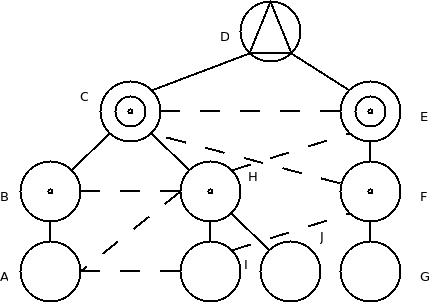
\includegraphics[width=0.5\textwidth]{Imagen/ejercicio10tema1.jpg}
\label{}
\end{figure}
\begin{center}
\begin{tabular}{| c | c | c | c | c | c | c | c | c | c | c |}
\hline
   & A & B  & C  & D  & E  & F  & G & H  & I  & J  \\\hline
 A & - & 15 & 15 & 10 & 3  & 5  & 4 & 10 & 5  & 1  \\\hline
 B &   & -  & 15 & 10 & 3  & 5  & 5 & 10 & 5  & 1  \\\hline
 C &   &    & -  & 10 & 20 & 30 & 1 & 1  & 5  & 2  \\\hline
 D &   &    &    & -  & 10 & 10 & 5 & 1  & 2  & 1  \\\hline
 E &   &    &    &    & -  & 5  & 5 & 25 & 10 & 5  \\\hline
 F &   &    &    &    &    & -  & 5 & 5  & 10 & 2  \\\hline
 G &   &    &    &    &    &    & - & 10 & 5  & 2  \\\hline
 H &   &    &    &    &    &    &   & -  & 5  & 2  \\\hline
 I &   &    &    &    &    &    &   &    & -  & 2  \\\hline
\end{tabular}
\end{center}
\textbf{1.} Rutas entre las siguientes centrales: A$\to$I, I$\to$G, A$\to$G, J$\to$G.\\
\begin{center}
\begin{tabular}{c c c c}
A$\to$I & AI  		& I$\to$G 	& IFG 		\\
 		& ABHI		&			& IHEFG		\\
 		& ABCHI		&			& IHCFG		\\
 		& 			&			& IHCDEFG	\\
A$\to$G & ABCFG  	& J$\to$G 	& JHEFG 	\\
 		& ABCDEFG	&			& JHCFG		\\
 		& 			&			& JHCDEFG	\\
\end{tabular}
\end{center}
\textbf{2.} Tráfico ofrecido y cursado en la sección directa CE/EC.\\
\begin{gather*}
TO_{CE}=TO_{CEpropio}+TO_{HEdesb}+TO_{BE}+TO_{AE}\\
TO_{HE}=TO_{HEpropio}+TO_{IFdesb}+TO_{HF}+TO_{HG}+TO_{JE}+TO_{JF}+TO_{JG}\\
TO_{IF}=TO_{IFpropio}+TO_{IG}=15E\\
TO_{HE}=50.5E\\
TO_{CE}=31.05E\\
TC_{CE}=TO_{CE}(1-P_B)=30.7395E\\
TO_{EC}=TO_{ECpropio}+TO_{FC'desb}+TO_{EB}+TO_{EA}\\
TO_{FC'}=TO_{FCpropio}+TO_{FB}+TO_{FA}+TO_{GC}+TO_{GB}+TO_{GA}=50E\\
TO_{EC}=31E\\
TC_{EC}=30.69E
\end{gather*}
\end{exercise}
\begin{exercise}[11]
En la comunidad Autónoma de Andalucía (con 8 provincia), existe una central secundaria en cada provincia para cursar el tráfico provincial, y solo una central terciaria situada en Sevilla para cursar el tráfico interprovincial. Ahí es precisamente donde se sitúa el proveedor de servicios de Internet o ISP. Asumamos que cada provincia está compuesta por 10 localidades (es un escenario ficticio pero es para poder simplificar el ejercicio), y en cada una de ellas se encuentra situada una central primaria, para cursar el tráfico local. Asimismo, cada localidad está formada por una serie de barrios, y en cada uno de ellos existe una central local con capacidad para 2000 líneas.\\
La arquitectura de la red es la siguiente. Todas las centrales locales bajo la misma central primaria se encuentran conectadas mediante enlaces directos para cursar, en primera instancia, el tráfico local. La probabilidad de desbordamiento en estas secciones directas es del 10\% . Además, cada central local se encuentra conectada a la central secundaria de la que depende jerárquicamente
\end{exercise}
\subsection{Multiplexación y metodos de acceso}
\begin{figure}[H]
\centering
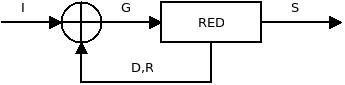
\includegraphics[width=0.5\textwidth]{Imagen/diametodosacceso.jpg}
\caption{Diagrama de Métodos de Acceso}
\end{figure}
\begin{itemize}
\item I: Tráfico. siempre ha de ser menor que 1.
\item G: Tráfico ofrecido a la red.
\item S: Eficiencia de la red.
\item R: Retransmisiones.
\item D: Retardo en la transmisión.
\end{itemize}
I, G, S, R han de estar normalizados a la capacidad de la red. D en cambio ha de estar normalizado a la velocidad de la red. En caso de que no haya congestión S será igual a I. $\sfrac{S}{G}$ expresa la probabilidad media de transmitir paquetes con éxito. $\sfrac{G}{S}$ en cambio el número de retransmisiones medias necesarias para transmitir un paquete con éxito.
\subsubsection{Aloha puro}
\begin{enumerate}
\item Si un terminal quiere transmitir, transmite y espera un ACK del destino.
\item Si no recibe el ACK de confirmación espera un tiempo aleatorio entre uno y k para retransmitir.
\end{enumerate}
\begin{align}
G&=S+R\\
\frac{S}{G}&=e^{-2g}\\
D=(\frac{G}{S}-1)(\frac{k+1}{2}+1+2a+w)+a+1 &
\begin{cases}
a\text{ tiempo de propagación del paquete}\\
w\text{ tiempo de generación del ACK}\\
k\text{ limite máximo de la espera}
\end{cases}
\end{align}
La eficiencia máxima que se puede obtener con ALOHA puro es $S_{max}=0.18$ este valor se produce para G=0.5.\\
\begin{example}[ALOHA puro]
Tenemos un canal de comunicaciones de capacidad 9600bps, y enviamos paquetes de 100 bits. Se sabe que se generan 10.67$\sfrac{paquetes}{segundo}$ y que el tráfico total son 14.4$\sfrac{paquetes}{segundo}$.
\begin{gather*}
C=\frac{9600}{100}\\
D=(\frac{G}{S}-1)(\frac{k+1}{2}+1+2a+w)+a+1\\
I=S=\frac{10.67\sfrac{paq}{s}}{96\sfrac{paq}{s}}=0.11\\
G=\frac{14.4\sfrac{paq}{s}}{96\sfrac{paq}{s}}=0.15\\
\frac{G}{S}=\frac{0.15}{0.11}=1.35\text{ transmisiones por paquete}\\
R=\frac{G}{S}-1=0.35\text{ retransmisiones por paquete}\\
\frac{S}{G}=\frac{0.11}{0.15}=0.74=74\%
\end{gather*}
\end{example}
\subsubsection{Aloha distribuido}
\begin{align}
S=Ge^{-2G(1+a)}\\
D=(e^{-2G(1+a)}-1)(\frac{k+1}{2}+1+2a+w)+a+1
\end{align}
\subsubsection{Aloha ranurado}
El tiempo se divide en ranuras y solo se transmite al comienzo de las ranuras reduciendo el tiempo de colisión.
\begin{align}
S=Ge^{-G}\\
D=(e^{-G}-1)(\frac{k+1}{2}+1.5+2a+w)+a+1.5
\end{align}
La eficiencia máxima que se puede obtener con ALOHA puro es $S_{max}=0.36$ este valor se produce para G=1.\\
\subsubsection{CSMA}
\begin{itemize}
\item Antes de transmitir se escucha el canal.
\item Si no hay nadie transmitiendo se transmite.
\item Si el canal está ocupado:
\subitem No persistente: Se espera un tiempo aleatorio y se escucha el canal. $S=\frac{G}{G+1}$
\subitem 1-persistente: Se escucha hasta que el canal esté libre. $S=\frac{G(1+G)e^{-G}}{G+e^{-G}}$ este tiene una eficiencia máxima del 55\%.
\subitem p-persistente: Se espera con una probabilidad 1-py se transmite con probabilidad p.
\end{itemize}
\subsubsection{Ejercicios}
\begin{exercise}[4]
Se dispone de una red de terminales de comunicaciones que acceden a un controlador central según un esquema ALOHA ranurado con parámetro k=5. La capacidad del canal es de 56 Kbps y cada terminal manda en media 1 paquete de 1000 bits de duración cada 100 segundos. La distancia de cada uno de los terminales al controlador es de 3km y el tiempo que tarda en generar un paquete ACK es de 10 mseg.\\
\textbf{1.} ¿Cuántos terminales pueden compartir el canal si el rendimiento del sistema es la mitad del máximo posible?\\
\begin{gather*}
S=I=\frac{S_{max}}{2}=0.18\\
I=\frac{Na_o}{C}\\
C=56Kbps=56*1024=57344bbps\\
a_o=\frac{1000bits}{100s}=10bps\\
N=1032terminales
\end{gather*}
\textbf{2.} ¿Cuantos intentos hay que hacer en media para transmitir con éxito un paquete?\\
Para obtener el valor de G haremos una tabla donde por prueba y error intentaremos aproximarnos al valor de S=0.18.
\begin{gather*}
S=Ge^{-G}\\
\frac{G}{S}=\frac{0.2255}{0.18}=1.25 intentos
\end{gather*}
\begin{center}
\begin{tabular}{c | c}
G & S \\\hline
0.1 & 0.009\\
0.2 & 0.1637\\
0.3 & 0.22\\
0.25 & 0.19\\
0.2255 & 0.18\\
\end{tabular}
\end{center}
Como se puede ver tanto 0.2 como 0.3 se aproximan bastante y serian suficientemente buenos para un examen.\\
\textbf{3.} ¿Cuántos servidores están desocupados en media?\\
\begin{gather*}
D=1.5+a+(\frac{G}{S}-1)(1.5+2a+w+\frac{1+k}{2})=2.86\\
t_a=\frac{d}{c}=\frac{3*10^3}{3*10^8}=10^{-5}seg\\
m=\frac{1000}{56*1024}=0.0174\sfrac{seg}{paq}\\
a=\frac{t}{m}=57.34*10^{-3}\\
w=\frac{t_{ACK}}{m}=1.5734
\end{gather*}
\end{exercise}

\subsection{Ejercicios}
\begin{exercise}[1]
Se desea estudiar el envío de paquetes de 128 bytes en una red de conmutación de paquetes con encaminamiento fijo. El enlace entre nodos tiene una capacidad de 64kbps.\\
\textbf{1.} ¿Qué modelo de sistema de colas se puede aplicar?.\\
Se trata de un sistema M/M/1\\
\textbf{2.} ¿Cuál es el número medio de paquetes servidos por segundo?\\
\[\mu=8\sfrac{KB}{s}\frac{1Paquete}{128Bytes}=62.5\sfrac{Paquetes}{s}\]
\textbf{3.} ¿Cuál es el número medio de paquetes por segundo que un nodo puede aceptar para que el tiempo medio de espera en el buffer sea igual a 10 segundos?\\
\begin{gather*}
W_q=\frac{\rho}{\mu(1-\rho)}=10s\\
\rho=\frac{A_c}{c}=A_o=\frac{\lambda}{\mu}\to \lambda=\rho \mu\\
W_q=\frac{\rho}{\mu(1-\rho)}\to\rho=\frac{W_q \mu}{1+W_q\mu}=0.9984\\
\lambda=62.4\sfrac{Paquetes}{s}
\end{gather*}
\textbf{4.} ¿Cuánta memoria en media se estará ocupando en el nodo?\\
\[\text{Memoria}=L_q128=128\frac{\rho^2}{1-\rho}=79.744kB=637.9kb\]
\[L_q=623 \text{ Paquetes en cola de media}\]
\end{exercise}
\begin{exercise}[2]
Un conmutador monoproceso de servicio 16 horas al día FCFS(First Come First Serve) a un conjunto de usuarios. El patrón de llegadas programadas es poissonianode media 20 programas/día y la distribución de tiempo de CPU  de cada programa es exponendial de media 30 minutos.\\
\textbf{1.} ¿Cuál será el factor de utilización de la CPU?\\
Se trata de un M/M/1 con lo cual $\rho=A_o$.\\
\[\rho=\frac{\lambda}{\mu}=\frac{20*30}{60*16}=0.625=62.5\%\]
\textbf{2.} Se reciben quejas de los usuarios, ¿a qué puede ser debido?\\
\[W_q=\frac{\rho}{\mu(1-\rho)}=50\text{ minutos}\]
Se está casi el doble de tiempo en cola que dentro del servidor. Este será el motivo de queja mayoritario.\\
\textbf{3.} Se decide colocar en paralelo tantas CPUs como sean necesarias para garantizar que el tiempo medio de espera en cola sea inferior o como máximo de 10 minutos. ¿Cuántos deben colocarse?\\
\begin{gather*}
A_c=A_o=0.625\\
\rho=\frac{A_c}{c}=\frac{A_o}{c}\\
W_q=E(s)\frac{C(A_o,c)}{c(1-\rho)}
\end{gather*}
Hallaremos la respuesta por prueba y error:
\begin{center}
\begin{tabular}{c|c|c|c}
CPU & $\rho$ & $C(A_o,c)$ & $W_q$ \\\hline
2 & 0.3125 & 0.15 & 3.27 min\\
3 & 0.208 & 0.03 & 0.38 min
\end{tabular}
\end{center}
Como se puede ver en la tabla con solamente añadir un segundo servidor se puede conseguir el objetivo de estar menos de 10 minutos en la cola.\\
\textbf{4.} ¿Es conveniente instalar 2 CPUs que se repartan los usuarios de forma que cada una atienda por separado a la mitad de las peticiones recibidas?\\
Aquí se puede ver que vuelve a ser un sistema M/M/1 con $\lambda=10\sfrac{programas}{dia}$.
\begin{gather*}
\rho=A_o=\frac{\lambda}{\mu}=\frac{30*10}{60*16}=0.3125\\
W_q=E(s)\frac{\rho}{1-\rho}=13.63 \text{ minutos de espera de media}
\end{gather*}
Como se puede ver 13.63\textgreater \textgreater 3.27. Con esto se demuestra que los sistemas de cola única son mucho más eficientes.
\end{exercise}
\begin{exercise}[3]
Los usuarios de una población infinita demandan poisonianamente con tasa 0.1 demandas/segundo un recurso sin cola de espera, con c servidores idénticos. El servicio demandado es exponencial de media E(s). Se desea garantizar que el tiempo de respuesta no sea superior a 10 segundos para al menos el 80\% de los usuarios, y se quiere perder menos del 15\% de los usuarios.\\
\textbf{1.} Calcular E(s) para cumplir con los valores requeridos.\\
\begin{gather*}
p(t<10s)=1-e^{-10\mu}=0.8 \to \mu=0.16\sfrac{\text{demandas}}{\text{segundo}}\\
E(s)=\frac{1}{\mu}=6.25\sfrac{\text{s}}{\text{demanda}}
\end{gather*}
\textbf{2.} ¿Cuántos servidores es necesario colocar?\\
Con $A_o=\sfrac{\lambda}{\mu}=0.625E$ y $P_B<15\%$ miramos en la gráfica de Erlang B y obtenemos que el número de servidores c ha de ser mayor o igual a 2.\\
\textbf{3.} ¿Cuántos servidores están desocupados en media?\\
$L=L_s=A_c=A_o(1-P_B)=0.53125$ usuarios de media en el sistema con lo cual hay 1.46875 servidores libres de media en el sistema.
\end{exercise}
\begin{exercise}[4]
Se dispone de una red de terminales de comunicaciones que acceden a un controlador central según un esquema ALOHA ranurado con parámetro k=5. La capacidad del canal es de 56 Kbps y cada terminal manda en media 1 paquete de 1000 bits de duración cada 100 segundos. La distancia de cada uno de los terminales al controlador es de 3km y el tiempo que tarda en generar un paquete ACK es de 10 mseg.\\
\textbf{1.} ¿Cuántos terminales pueden compartir el canal si el rendimiento del sistema es la mitad del máximo posible?\\
\begin{gather*}
S=I=\frac{S_{max}}{2}=0.18\\
I=\frac{Na_o}{C}\\
C=56Kbps=56*1024=57344bbps\\
a_o=\frac{1000bits}{100s}=10bps\\
N=1032terminales
\end{gather*}
\textbf{2.} ¿Cuantos intentos hay que hacer en media para transmitir con éxito un paquete?\\
Para obtener el valor de G haremos una tabla donde por prueba y error intentaremos aproximarnos al valor de S=0.18.
\begin{gather*}
S=Ge^{-G}\\
\frac{G}{S}=\frac{0.2255}{0.18}=1.25 intentos
\end{gather*}
\begin{center}
\begin{tabular}{c | c}
G & S \\\hline
0.1 & 0.009\\
0.2 & 0.1637\\
0.3 & 0.22\\
0.25 & 0.19\\
0.2255 & 0.18\\
\end{tabular}
\end{center}
Como se puede ver tanto 0.2 como 0.3 se aproximan bastante y serian suficientemente buenos para un examen.\\
\textbf{3.} ¿Cuántos servidores están desocupados en media?\\
\begin{gather*}
D=1.5+a+(\frac{G}{S}-1)(1.5+2a+w+\frac{1+k}{2})=2.86\\
t_a=\frac{d}{c}=\frac{3*10^3}{3*10^8}=10^{-5}seg\\
m=\frac{1000}{56*1024}=0.0174\sfrac{seg}{paq}\\
a=\frac{t}{m}=57.34*10^{-3}\\
w=\frac{t_{ACK}}{m}=1.5734
\end{gather*}
\end{exercise}
\begin{exercise}[5]
La red telefónica de la figura tiene una probabilidad de pérdidas en las secciones finales del 1\% y una probabilidad de desbordamiento en las secciones directas del 10\% .
\begin{figure}[H]
\centering
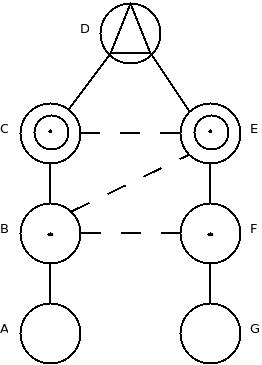
\includegraphics[width=0.5\textwidth]{Imagen/ejercicio5tema1.jpg}
\label{}
\end{figure}
La matriz de tráfico (simétrica) en Erlangs es la siguiente:
\begin{center}
\begin{tabular}{| c | c | c | c | c | c | c | c |}
\hline
   & A & B & C & D & E & F & G \\\hline
 A & - & 10 & 15 & 5 & 2 & 1 & 1 \\\hline
 B &   & - & 50 & 15 & 6 & 3 & 2 \\\hline
 C &   &   & - & 80 & 30 & 10 & 5 \\\hline
 D &   &   &   & - & 90 & 15 & 5 \\\hline
 E &   &   &   &   & - & 60 & 18 \\\hline
 F &   &   &   &   &   & - & 12 \\\hline
\end{tabular}
\end{center}
Se pide:\\
\textbf{1.} Indicar los caminos que comunican los nodos E y A.\\
\begin{center}
\begin{tabular}{c c c c}
E$\to$A & EBA  		& A$\to$E 	& ABE 	\\
 		& EDCBA		&			& ABCE	\\
 		& 			&			& ABCDE	\\
\end{tabular}
\end{center}
\textbf{2.} Calcular el tráfico ofrecido y cursado en la sección directa C$\to$E.\\
\begin{gather*}
TO_{C\to E}=TO_{CEpropio}+TO_{BEdesb}+TO_{BFdesb}+TO_{CF}+TO_{CG}=\\
30+0.8+0.7+10+5=46.5E\\
TO_{BE}=TO_{BEpropio}+TO_{AE}=8E\\
TO_{BEdesb}=TO_{BE}P_d=TO_{BE}0.1=0.8E\\
TO_{BF}=TO_{BFpropio}+TO_{BG}+TO_{AF}+TO_{AG}=7E\\
TO_{BFdesb}=TO_{BF}P_d=TO_{BF}0.1=0.7E\\
TC_{C\to E}=TO_{C\to E}(1-P_D)=41.85E
\end{gather*}
\textbf{3.} Considerando solo el tráfico saliente de A y sabiendo que la probabilidad de que la duración de la llamada sea superior a 5 minutos es de 0.08205, ¿cuál es la duración media de la llamada?\\
Se trata de un sistema con bloqueo M/M/c/c con $A_{oA}=34E=\frac{\lambda}{\mu}$.
\begin{gather*}
P(W>5min)=\int_{5}^{\infty}\mu e^{-\mu t}dt=-e^{-\mu t}\Big|_{5}^{\infty}=0.08205\\
\mu=0.5\sfrac{llamadas}{minuto}\to E(s)=2\sfrac{minutos}{llamada}
\end{gather*}
\textbf{4.} ¿Cuántos intentos de llamada se hacen en la hora cargada(HC)?\\
\begin{gather*}
A_{oA}=34E=\frac{\lambda}{\mu}\\
\mu=0.5\sfrac{llamadas}{minuto}\\
\lambda=34*0.5=17\sfrac{llamadas}{minuto}\\
\lambda_{HC}=17*60=1020\sfrac{llamadas}{hora}
\end{gather*}
\textbf{5.} Los registradores de la central A analizan las primeras cifras y encaminan las llamadas, pudiéndose modelar como un sistema M/M/c. Si el tiempo de ocupación de los registradores por cada llamada es de 6 segundos, ¿cuántos son necesarios para que la probabilidad de esperar más de 1 segundo sea de 0.008?\\
\begin{gather*}
E(s')=6\sfrac{segundos}{llamada}\to A'_o=\frac{\lambda}{\mu '}=1.7E\\
P(W_q>1s)=0.008=C(c,A'_o)e^-c\mu 'T(1-\rho)
\end{gather*}
Este apartado habrá que hacerlo por prueba y error hasta hallar el número de servidores necesarios para cumplir con las especificaciones. Se puede ver estas pruebas en la tabla:\\
\begin{center}
\begin{tabular}{c | c | c | c}
$C(c,A'_o)$ & c & $\rho$ & $P(W_q>1)$ \\\hline
0.7  & 2 & 0.85  & 0.6672 \\
0.1  & 4 & 0.425 & 0.0692 \\
0.008 & 6 & 0.283 & 0.00402
\end{tabular}
\end{center} 
De la tabla se puede observar que el número mínimo de registradores ha de ser 6.\\
\textbf{6.} ¿Cuál es el tiempo medio de espera en los registradores?\\
\[W_q=\frac{E(s)\rho}{1-\rho}=2.3682segundos\]
\end{exercise}
\begin{exercise}[6]
En un territorio de un país en vías de desarrollo, se ha decidido crear una nueva red telefónica digital. Para su planificación se han considerado los siguientes datos:
\begin{itemize}
\item Tras agrupar geográficamente los diferentes núcleos en entidades de población, resultando 83, se han obtenido 70 entidades  con 20000 habitantes, 10 con 60000, 2 con 1000000 y 1 (la capital) con 2000000
\item Se considera un grado inicial de penetración del servicio del 30\% (30 teléfonos por cada 100 habitantes). El incremento futuro de dicho porcentaje será absorbido por las correspondientes ampliaciones.
\item El tráfico total (entrante y saliente, excluyendo el local) por abonado se cifra en 20mE.
\item Se dispone de unidades locales de 6000 líneas.
\item Las centrales primarias tienen una capacidad para 3000E de tráfico total (entrante y saliente).
\item Existirá una central secundaria por cada 5 primarias y solo una central terciaria.
\item Sólo se establecen rutas finales, con una probabilidad de pérdida del 2\% (se puede aproximar la función de Erlang B por $B(A_o,c)=0.025\sfrac{A_o}{c}$.
\end{itemize}
Se desea conocer:\\
\textbf{1.} El número de unidades locales de conmutación necesarias.\\
\begin{gather*}
CL=(70\frac{20000}{6000}+10\frac{60000}{6000}+2\frac{1000000}{6000}+1\frac{2000000}{6000})30\%\\
CL=300\text{ centrales locales}
\end{gather*}
\textbf{2.} Los sistemas MIC de norma europea que permitirán la conexión de cada unidad local con su correspondiente primaria.\\
Cada unidad local genera $A_{oCL}=6000*0.02=120E$ con una probabilidad de pérdida del 2\% y utilizando la función Erlang B obtenemos:
\begin{gather*}
B(A_o,c)=0.025\sfrac{A_{oCL}}{c}=0.02\\
c=\frac{0.025A_{oCL}}{0.02}=150\text{ canales}\\
MIC=\frac{c}{30}=5\text{ sistemas MIC de norma europea}
\end{gather*}
\textbf{3.} El número de centrales primarias.\\
\[CP=\frac{300}{\frac{3000E}{6000*0.02E}}=12\text{ centrales primarias}\]
\textbf{4.} El número de centrales secundarias.\\
\[CS=\frac{12}{5}=2.4\to 3\text{ centrales secundarias}\]
\end{exercise}
\begin{exercise}[7]
Con motivo del cambio de numeración de 6/7 cifras a 8 se contempla la digitalización de la red telefónica de un país. Para ello, se realiza el diseño de la red basándose en los siguientes datos:
\begin{itemize}
\item La capacidad de las unidades locales (centrales urbanas) es de 40000 líneas.
\item La capacidad de las centrales de tránsito (primarias y secundarias) es de 40000 enlaces.
\item Las centrales locales de cada núcleo urbano se conectarán mediante secciones directas en malla (todas con todas) para cursar, en primera instancia el tráfico urbano.
\item Las centrales locales se conectarán a una de las centrales secundarias (ruta directa) para cursar, como primera alternativa, el tráfico interurbano y el internacional.
\item Cada central local se conectará a su correspondiente central primaria (ruta final), para el desbordamiento del tráfico anterior.
\item Cada central primaria se conectará a su secundaria jerárquica ( ruta final), constituyendo éstas entre si una red mallada.
\item Considerando despreciable la pérdida de tráfico originada por saturación de las diferentes centrales, se prevén, para los enlaces y correspondientes medios de transmisión unas probabilidades del 1\% de pérdidas y del 10\% de desbordamiento.
\item Se estima un tráfico por abonado de 100mE, desglosado del siguiente modo:
\subitem 10+0.015A mE para tráfico urbano, al 50\% entre entrante y saliente, siendo A el número de abonados del núcleo urbano en miles.
\subitem Resto para tráfico interurbano e internacional, que se distribuye al 50\% entre entrante y saliente.
\end{itemize}
OBSERVACIONES:
\begin{itemize}
\item Se considera despreciable el tráfico local (entre abonados de la misma central local).
\item Se puede aproximar la distribución Erlang-B por la expresión $B(c,A_o)=8.33*10^{-3}\sfrac{c}{A_o}$ para el 1\% y $B(c,A_o)=0.1\sfrac{c}{A_o}$ para el 10\%.
\item Considerar que las centrales de tránsito por cada llamada son necesarios dos enlaces, uno de entrada y otro de salida.
\end{itemize}
\textbf{1.} Eficiencia (E/enlace) de las rutas directas y finales.\\
\begin{gather*}
B(c,A_o)=8.33*10^{-3}\frac{c}{A_o}\sfrac{enlace}{E}=1\% \to 8.33*10^{-3}\frac{1}{\eta_{RF}}=1\% \\
\eta_{RF}=8.33*10^{-3}\frac{1}{1\%}=0.833\sfrac{E}{enlace}\\
B(c,A_o)=0.1\frac{c}{A_o}\sfrac{enlace}{E}=10\% \to 0.1\frac{1}{\eta_{RF}}=10\% \\
\eta_{RF}=0.1\frac{1}{10\%}=1\sfrac{E}{enlace}
\end{gather*}
\textbf{2.} Capacidad de tráfico (E)de las centrales primarias.\\
\begin{gather*}
C_CP=\frac{40000}{2}\eta_{RF}=16660E
\end{gather*}
\textbf{3.} Distribución, en las cenrales secundarias, entre enlaces de secciones directas y finales, y la capacidad de tráfico de dichas centrales.\\
\begin{gather*}
\begin{cases}
N_{RD}+N_{RF}=\frac{40000}{2}\\
N_{RD}\eta_{RD}=N_{RF}\eta_{RF}
\end{cases}
N_{RD}=17547enlaces\\
N_{RF}=2453enlaces\\
C_{CS}=N_{RD}\eta_{RD}+N_{RF}\eta_{RF}=19590E
\end{gather*}
\textbf{4.} Considerando una capacidad de 16000E y 19600E para las centrales primarias y secundarias, respectivamente, evaluar, para un núcleo de 3.5 millones de abonados, el número de centrales locales, primarias y secundarias necesario.\\
Asumiendo $C_{CP}=16000E$ y $C_{CS}=19600E$ y una población $A=3.5*10^6abonados$
\begin{gather*}
N_{CL}=\frac{A}{40000}=87.5\to88\text{ centrales locales}\\
N_{CP}=10\% a_o
\end{gather*}
\textbf{5.} Si se reserva el prefijo 0 para servicios especiales y el prefijo 9 para el acceso interurbano, estimar la capacidad (número máximo de abonados que admite) del nuevo plan de numeración. Considerar que si el número local es del tipo ZXXXXXXX, el número nacional de 10 dígitos se formará anteponiendo el prefijo 0X.\\
\myworries{Acabar el ejercicio}
\end{exercise}
\begin{exercise}[8]
En el servicio de cobro revertido automático (SCRA), también llamado "Línea 900", el cobro de la llamada se carga, de manera automática, al abonado llamado, y no al llamante. Un nuevo operador de telecomunicaciones pretende ofertar dicho servicio mediante la estructura de red de la figura.\\
%%Incluir imagen
\myworries{Incluir imagen del ejercicio}
El servicio funciona de la siguiente forma: cuando un usuario marca un número 900.XXX.XXX, se encamina la llamada a una central específica, que realiza la traducción de dicho número y transfiere la comunicación a este último número, al cual le carfa el coste de la llamada. En la planificación del servicio, se han tenido en cuenta las siguientes estimaciones de tráfico:
\begin{itemize}
\item Desde Madrid se originarán, en la Hora Cargada (HC) y para la SCRA, 12000 llamadas, de las que el 0.127\% superarán los 10 minutos.
\item El tráfico total dirigido al SCRA de toda España será 4 veces el originado en Madrid.
\item Para todas las rutas, la probabilidad de pérdida es del 1\%
\end{itemize}
OBSERVACIÓN: Puede aproximar la distribución Erlang-B por la expresión $B(c,A_o)=8.2*10^{-3}\sfrac{c}{A_o}$\\
NOTA: Una empresa puede tener múltiples núeros del tipo 9XX.XXX.XXX (por ejemplo, uno por provincia donde tenga una oficina( y tener, en cambio un único 900.XXX.XXX; al traducir este último, se optará por alguno de los anteriores en base a criterios preestablecidos (por ejemplo, el origen de la llamada).\\
Se desea:\\
\textbf{1.} Dibuje la arquitectura de la Red Inteligente que soporta dicho servicio, indicando claramente qué entidades funcionales aparecen y cuáles se corresponden con el dibujo de la figura.\\

\textbf{2.} Para la ruta de la provincia de Madrid: tráfico (en Erlangs), número de canales (o circuitos), número de sistemas MIC de norma europea.\\

\textbf{3.} Para cada una de las rutas de entrada en RTB: tráfico (en Erlangs), número de canales (o circuitos), número de sistemas de 8 MBps (E2 de 120 canales).\\
\myworries{hacer ejercicio}
\end{exercise}
\begin{exercise}[9]
En la red telefónica de la figura se muestran las rutas finales y las secciones directas. La probabilidad de bloqueo es del 1\% y una probabilidad de desbordamiento del 10\% . Sobre esta red, se le pide lo siguiente:
\begin{figure}[H]
\centering
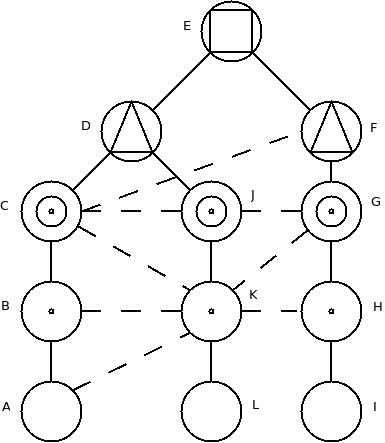
\includegraphics[width=0.5\textwidth]{Imagen/ejercicio9tema1.jpg}
\label{}
\end{figure}
\textbf{1.} Indique las rutas entre las siguientes centrales:\\
\begin{center}
\begin{tabular}{c c c c}
A$\to$L & AKL  		& L$\to$A 	& LKA 	\\
 		& ABKL		&			& LKJCBA	\\
 		& ABCKL		&			& LKJDCBA	\\
 		& ABCDJKL	&			& 	\\
A$\to$I & ABCFGHI  	& L$\to$I 	& LKHI 	\\
 		& ABCDEFGHI	&			& LKJGHI	\\
 		& 			&			& LKJDEFGHI	\\
I$\to$L & IHKL  	& 		 	&  	\\
 		& IHGKL		&			& 	\\
 		& IHGFEDJKL	&			& 	\\
\end{tabular}
\end{center}
\textbf{2.} Calcule el tráfico ofrecido y el tráfico cursado en la sección directa JC/CJ y en la sección final CD/DC.\\
\begin{center}
\begin{tabular}{| c | c | c | c | c | c | c | c | c | c | c | c | c |}
\hline
   & A & B  & C  & D  & E  & F  & G & H  & I  & J  & K  & L \\\hline
 A & - & 15 & 15 & 10 & 5  & 5  & 5 & 10 & 2  & 1  & 8  & 2 \\\hline
 B &   & -  & 15 & 10 & 4  & 5  & 5 & 10 & 2  & 1  & 9  & 1 \\\hline
 C &   &    & -  & 10 & 10 & 20 & 5 & 10 & 5  & 1  & 5  & 5 \\\hline
 D &   &    &    & -  & 10 & 10 & 5 & 1  & 1  & 1  & 0  & 1 \\\hline
 E &   &    &    &    & -  & 5  & 5 & 25 & 10 & 5  & 1  & 0 \\\hline
 F &   &    &    &    &    & -  & 5 & 5  & 10 & 5  & 1  & 1 \\\hline
 G &   &    &    &    &    &    & - & 10 & 5  & 10 & 5  & 5 \\\hline
 H &   &    &    &    &    &    &   & -  & 10 & 15 & 5  & 5 \\\hline
 I &   &    &    &    &    &    &   &    & -  & 10 & 5  & 5 \\\hline
 J &   &    &    &    &    &    &   &    &    & -  & 10 & 10 \\\hline
 K &   &    &    &    &    &    &   &    &    &    & -  & 10 \\\hline
\end{tabular}
\end{center}
Empezamos por calcular el tráfico ofrecido en un sentido y luego en el otro.
\begin{gather*}
TO_{CJ}=TO_{CJpropio}+TO_{AJ}+TO_{BJ}=3E\\
TO_{JC}=TO_{JCpropio}+TO_{KCdesb}+TO_{KBdesb}+TO_{KAdesb}+TO_{JA}+TO_{JB}\\
TO_{KC}=TO_{KCpropio}+TO_{LC}=10\\
TO_{KB}=TO_{KBpropio}+TO_{LB}=10\\
TO_{KA}=TO_{KApropio}+TO_{LA}=10\\
TO_{JC}=1+1+1+1+1+1=6\\
TO_{CD}=TO_{CDpropio}+TO_{CFdesb}+TO_{CJdesb}+TO_{CKdesb}+TO_{CE}+TO_{AD}+TO_{AE}+TO_{BD}+TO_{BE}\\
TO_{CF}=TO_{CFpropio}+TO_{CG}+TO_{CH}+TO_{CI}+TO_{BF}+TO_{BG}+TO_{BH}+TO_{BI}+TO_{AF}+TO_{AG}+\\
+TO_{AH}+TO_{AI}=84E\\
TO_{CJ}=3E\\
TO_{CK}=TO_{CKpropio}+TO_{BKdesb}+TO_{CL}\\
TO_{BK}=TO_{BKpropio}+TO_{AKdesb}+TO_{BL}\\
TO_{AK}=TO_{AKpropio}+TO_{AL}=10E\\
TO_{BK}=11E\\
TO_{CK}=11.1E\\
TO_{CD}=10+8.4+0.3+1.11+10+10+5+10+4=58.81E\\
TO_{DC}=TO_{DCpropio}+TO_{FCdesb}+TO_{JCdesb}+TO_{EC}+TO_{DB}+TO_{EB}+TO_{DA}+TO_{EA}\\
TO_{FC}=TO_{FCpropio}+TO_{GC}+TO_{HC}+TO_{IC}+TO_{FB}+TO_{GB}+TO_{HB}+TO_{IB}+TO_{FA}+TO_{GA}+\\
+TO_{HA}+TO_{IA}=84E\\
TO_{JC}=6E\\
TO_{DC}=10+8.4+0.6+10+10+5+10+4=58E
\end{gather*}
Para terminar calcularemos el tráfico cursado en cada uno de los tramos como $TC=TO(1-P_B)$ siendo $P_B$ la probabilidad de bloqueo en las rutas finales y la probabilidad de desbordamiento en las secciones directas.
\begin{gather*}
TC_{CJ}=TO_{CJ}(1-P_D)=2.7E\\
TC_{JC}=TO_{JC}(1-P_D)=5.4E\\
TC_{CD}=TO_{CD}(1-P_B)=58.22E\\
TC_{DC}=TO_{DC}(1-P_B)=57.42E
\end{gather*}
\end{exercise}
\begin{exercise}[10]
Utilice la red de la figura y la tabla adjunta (que es simétrica) para contestar a las siguientes preguntas:\\
NOTA: La probabilidad de pérdidas en ruta final es del 1 \% y la probabilidad de desbordamiento en secciones directas es del 10\% .
\begin{figure}[H]
\centering
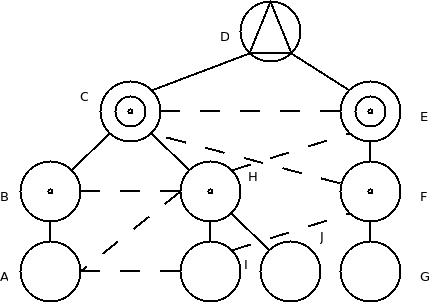
\includegraphics[width=0.5\textwidth]{Imagen/ejercicio10tema1.jpg}
\label{}
\end{figure}
\begin{center}
\begin{tabular}{| c | c | c | c | c | c | c | c | c | c | c |}
\hline
   & A & B  & C  & D  & E  & F  & G & H  & I  & J  \\\hline
 A & - & 15 & 15 & 10 & 3  & 5  & 4 & 10 & 5  & 1  \\\hline
 B &   & -  & 15 & 10 & 3  & 5  & 5 & 10 & 5  & 1  \\\hline
 C &   &    & -  & 10 & 20 & 30 & 1 & 1  & 5  & 2  \\\hline
 D &   &    &    & -  & 10 & 10 & 5 & 1  & 2  & 1  \\\hline
 E &   &    &    &    & -  & 5  & 5 & 25 & 10 & 5  \\\hline
 F &   &    &    &    &    & -  & 5 & 5  & 10 & 2  \\\hline
 G &   &    &    &    &    &    & - & 10 & 5  & 2  \\\hline
 H &   &    &    &    &    &    &   & -  & 5  & 2  \\\hline
 I &   &    &    &    &    &    &   &    & -  & 2  \\\hline
\end{tabular}
\end{center}
\textbf{1.} Rutas entre las siguientes centrales: A$\to$I, I$\to$G, A$\to$G, J$\to$G.\\
\begin{center}
\begin{tabular}{c c c c}
A$\to$I & AI  		& I$\to$G 	& IFG 		\\
 		& ABHI		&			& IHEFG		\\
 		& ABCHI		&			& IHCFG		\\
 		& 			&			& IHCDEFG	\\
A$\to$G & ABCFG  	& J$\to$G 	& JHEFG 	\\
 		& ABCDEFG	&			& JHCFG		\\
 		& 			&			& JHCDEFG	\\
\end{tabular}
\end{center}
\textbf{2.} Tráfico ofrecido y cursado en la sección directa CE/EC.\\
\begin{gather*}
TO_{CE}=TO_{CEpropio}+TO_{HEdesb}+TO_{BE}+TO_{AE}\\
TO_{HE}=TO_{HEpropio}+TO_{IFdesb}+TO_{HF}+TO_{HG}+TO_{JE}+TO_{JF}+TO_{JG}\\
TO_{IF}=TO_{IFpropio}+TO_{IG}=15E\\
TO_{HE}=50.5E\\
TO_{CE}=31.05E\\
TC_{CE}=TO_{CE}(1-P_B)=30.7395E\\
TO_{EC}=TO_{ECpropio}+TO_{FC'desb}+TO_{EB}+TO_{EA}\\
TO_{FC'}=TO_{FCpropio}+TO_{FB}+TO_{FA}+TO_{GC}+TO_{GB}+TO_{GA}=50E\\
TO_{EC}=31E\\
TC_{EC}=30.69E
\end{gather*}
\end{exercise}
\begin{exercise}[11]
En la comunidad Autónoma de Andalucía (con 8 provincia), existe una central secundaria en cada provincia para cursar el tráfico provincial, y solo una central terciaria situada en Sevilla para cursar el tráfico interprovincial. Ahí es precisamente donde se sitúa el proveedor de servicios de Internet o ISP. Asumamos que cada provincia está compuesta por 10 localidades (es un escenario ficticio pero es para poder simplificar el ejercicio), y en cada una de ellas se encuentra situada una central primaria, para cursar el tráfico local. Asimismo, cada localidad está formada por una serie de barrios, y en cada uno de ellos existe una central local con capacidad para 2000 líneas.\\
La arquitectura de la red es la siguiente. Todas las centrales locales bajo la misma central primaria se encuentran conectadas mediante enlaces directos para cursar, en primera instancia, el tráfico local. La probabilidad de desbordamiento en estas secciones directas es del 10\% . Además, cada central local se encuentra conectada a la central secundaria de la que depende jerárquicamente mediante secciones directas con probabilidad probabilidad de desbordamiento del 15\%, para cursar,en primera instancia, todo el tráfico provincial e interprovincial. Cada central local se conecta por sección final a su central primaria. A su vez, cada central primaria se conecta mediante sección final a su central secundaria y cada central secundaria se conecta, por sección final a su central terciaria, formando de esta forma la ruta final, cuya probabilidad de bloqueo es del 1\%(asuma que si se bloquea una llamada, se bloquea en la última de las secciones). Considere también despreciable el tráfico local entre abonados de la misma central local.\\
Se ofrece una tarifa plana entre las 18:00 y las 8:00 de la mañana, para aprovechar el periodo donde menos tráfico vocal se cursa.\\
Se ha medido el siguiente tráfico por ususario en este escenario:
\begin{itemize}
\item 2 llamadas locales en la hora cargada, de 144 segundos de duración.
\item 1 llamada provincial o interprovincial en la hora cargada de 450 segundos de duración.
\item La distribución entre llamadas provinciales e interprovinciales es de 30\% y 70\%, respectivamente.
\item 1 llamada de datos de 42 minutos de duración.
\end{itemize}
\textbf{NOTA:} Para los apartados 3 y 4 (y solo para ellos) utilize las siguientes aproximaciones de la Erlang-B: $B(c,A_o)=0.01=\sfrac{A_o}{85c}$; $B(c,A_o)=0.1=\sfrac{A_o}{102c}$ y para la Erlang-C: $C(c,A_o)=0.01=\sfrac{7A_o}{c}$; $C(c,A_o)=0.1=\sfrac{53A_o}{c}$.\\
Se le pide que dimensione alguno de los enlaces de la red anterior:\\
\textbf{1.} Calcule el número de sistemas MIC de norma Europea en el enlace entre la central local y la central primaria.\\
\textbf{2.} Calcule el número de barrios por localidad sabiendo que la capacidad de la central primaria es 1090E\\
\textbf{3.} ¿Cuántos canales duplex serían necesarios para conectar la central primaria y su secundaria jerarquica?\\
\textbf{4.} El enlace entre las centrales secundarias y su terciaria se realiza mediante SDH. Calcule la jerarquía mínima SDH  necesaria para cursar todo el tráfico.\\
\textbf{5.} ¿Se podría utilizar SNCP en el enlace anterior? Razone su respuesta.
\end{exercise}
%% Tema 3
%\section{Transmisión de datos en banda ancha}
La banda ancha surge de la necesidad de cambiar la utilidad de las redes clásicas, es decir, adaptarse a las nuevas necesidades. Ahora las redes se usan más para la transmisión de datos que de voz.\\
Las redes se dividirán en:
\begin{itemize}
\item Red de acceso, conecta al usuario con la red.
\item Red troncal, secciones internas de las grandes redes de los proveedores de internet(ISP).
\end{itemize}
Al principio se optó por opciones como la Jerarquía Digital Plexincrona (PDH). Los sistemas MIC agrupan canales de 64kbps. El sistema MIC de norma europea agrupa 30 canales produciendo 2Mbps de transmisión y el americano 24 canales produciendo 1.5Mbps de transmisión.
\subsection{RDSI}
La Red Digital de Servicios Integrados(RDSI) es la siguiente evolución y ofrece dos canales por terminalque se podrán utilizar de la forma que cada uno decida. Este sistema tiene un latencia muy baja que aún no se ha podido igualar. Se utiliza TDM con un envío de un paquete de 8 bits cada 125 microsegundos.
\subsubsection{Estructura RDSI}
Como se puede ver en la imagen la estructura del RDSI es muy simple. La sección del ISP termina en TR1 que es la roseta de entrada a casa.
\begin{figure}[htp]
	\centering
	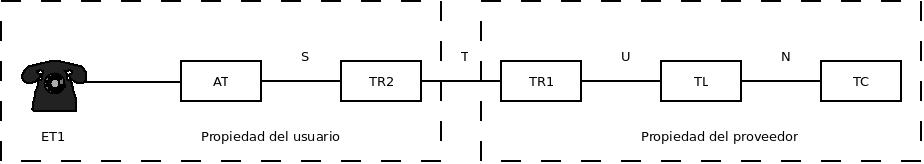
\includegraphics[width=\textwidth]{Imagen/diaRDSI.jpg}
	\caption{Estructura del sistema RDSI}
	\label{}
\end{figure}
Las difierentes piezas de la estructura son:
\begin{itemize}
	\item ET1: estación terminal. Con acceso básico podrían colocarse 2 terminales. estos son ordenadores, telefonos, etc.
	\item AT: este módulo se utiliza para adaptar telefonos analógicos al sistema digital. Este no siempre es necesario.
	\item TR2: una centralita de distribución, separa los canales para los diferentes terminales. No siempre hay uno
	\item TR1: roseta de entrada. Primer elemento perteneciente al ISP.
	\item TL y TC: son parte de la central local.
\end{itemize}
Las interfaces que conectan los anteriores son:
\begin{itemize}
	\item Interfaz S: 192kbps
	\item Interfaz T
	\item Interfaz U: 160kbps en acceso básico y 2mbps (europa), 1.5mbps (américa) en acceso primario.
	\item Interfaz N
\end{itemize}
Las interfaces S y T presentan la peculiaridad de ser iguales electricamente, es decir en caso de que no halla un TR2 la estación terminal se puede conctar directamente a la roseta. Esto no quita que en caso necesario las modulaciones o accesos multiples se puedan diferenciar.\\
\subsubsection{Accesos}
Los diferentes accesos se configuran en función de la configuración de diferentes canales.
\begin{itemize}
	\item Canal B: Transmite infromación a una velocidad de 64kbps.
	\item Canal D: Es un canal de señalización que va entre 16 y 64 kbps.
	\item Canal H: Transmite información a una velocidad superior a 64kbps.
\end{itemize}
Un acceso básico incluye dos canales B y un canal D (a 16kbps). Un acceso primario coincide con los sistemas MIC del sistema PDH. El acceso primario se constituye de 30 canales B y un canal D (a 64kbps) en europa y 23 canales B en américa.
\subsection{Banda ancha en núcleo de abonado xDSL}
Utilización del bucle de abonado más allá del telefono. Hace uso de modulaciones multiportadora adaptada. Se analiza el canal y se diseña en que frecuencias se utilizan que modulaciones para utilizar mejor el ancho de banda. En algunos casos por la cercania entre bandas es necesaria la utilización de cancelación de ecos.
\subsection{SDH}
Conjunto jerárquico de estructuras digitales de transporte de cargas adaptadas sobre redes de transmisión física". Se trata de una técnica de multiplexación utilizada normalmente en los sistemas de fibra óptica. Ha sido adaptado también a sistemas de cable coaxial.\\
El SDH utiliza como unidad básica el STM-1 (Módulo de Transferencia Sincrona). en la figura se puede ver la estructura lógica de un STM-1.
\begin{figure}[H]
\centering
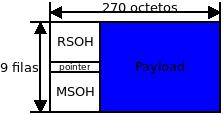
\includegraphics[width=0.7\textwidth]{Imagen/diaSTM1.jpg}
\caption{Estructura lógica de la trama STM-1}
\label{}
\end{figure}
\begin{itemize}
	\item Payload: Donde se guardan los datos enviados por los usuarios.
	\item RSOH: Cabezera de regeneración (al ser fibra hey que regenerar la señal cada poco espacio. CRC's, etc.
	\item MSOH: Cabezera de multiplexación, número de cargas, posición de cada una de ellas, etc.
	\item Pointer: Puntero al inicio de la carga util.
\end{itemize}
\subsubsection{Estructura de la multiplexación en SDH}
En la siguiente figura se puede ver la estructura seguida para la multiplexación de los diferentes contenedores de carga.
\begin{figure}[H]
\centering
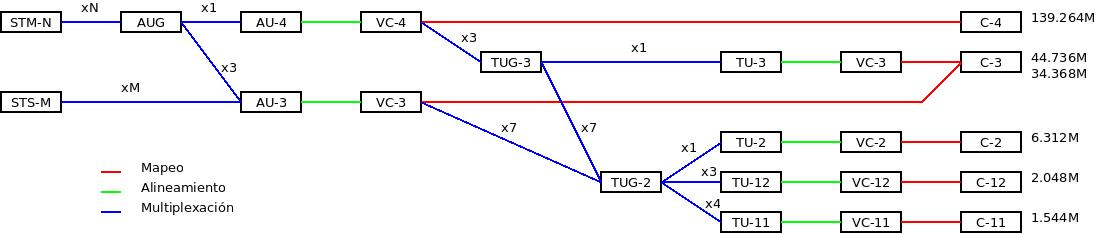
\includegraphics[width=\textwidth]{Imagen/diamuxSDH.jpg}
\caption{Estructura de la multiplexación en SDH}
\label{}
\end{figure}
\begin{itemize}
	\item C-x: Contenedor número x. Espacio de la trama dedicado a datos, se mide en Mbps. Un C-4 ocupa todo el espacio de payload de un STM-1.
	\item VC-x: Contenedor Virtual es un C-x con información del contenido del mismo. POH+C-x=VC-x
	\item AU-x: Unidad administrativa. Incluye un puntero a los contenedores virtuales
	\item TU-x: Unidad Tributaria, incluye información de la tarificación.
	\item TUG-x: Unidad Tributaria y de Gestión.
	\item AUG: Unidad Administrativa y de gestión.
	\item STS: es la unidad básica de la adaptación de SDH para el cable coaxial, similar al STM para la fibra óptica.
	\item STM: Módulo de Transferencia Síncrona.
\end{itemize}
El acto de mapear se da en el paso de un contenedor a su contenedor virtual. El alineamiento de los diferentes contenedores virtuales se produce para la obtención de unidades administrativas y tributarias. La multiplexación se produce al juntar todos los sistemas menores dentro de los STM.\\
Dentro de un STM-1 se pueden contener los siguientes contenedores:
\[STM-1=
\begin{cases}
63, & \text{c-12}\\
21, & \text{c-2}\\
3, & \text{c-3}\\
1, & \text{c-4}
\end{cases}
\]
\subsubsection{SNCP SubNetwork Connection Protection}
\subsection{Ejercicios}
\begin{exercise}[1]
Se pretende unir Madrid con Barcelona mediante un enlace SDH-STM1 (155520 Mbps) que se va a rellenar con tramas E1(2048 kbps). Se quiere saber:\\
\textbf{1.} ¿Qué tipo de contenedor se deberá utilizar?\\
Una trama E1 se empaqueta exactamente en un contenedor C-12, que a su vez se empaqueta en un contenedor virtual VC-12.\\
\textbf{2.} ¿Cuántas tramas E1 cabrían en un STM1?\\
En una supertrama STM1 caben 63 contenedores C-12.
\end{exercise}
\begin{exercise}[2]
Se dispone de un anillo de fibra óptica sobre el que se ha establecido una red SDH con enlaces a nivel jerárquico STM-16 entre tres ciudades: A, B y C. Queremos establecer el siguiente tráfico: A-B: 2VC4, A-C: 2VC4, B-C: 6VC4.\\
1. ¿Cuál sería la protección a elegir si queremos proteger solo el tráfico entre A y B? Dibuje el esquema de protección utilizada\\
2. ¿Cuál sería la protección a elegir si queremos proteger todo el tráfico? Dibuje el esquema de protección utilizada\\
\end{exercise}
\begin{exercise}[3]
La compañía propietaria de los bucles de abonado de una población de 3500$\sfrac{habitantes}{km^2}$desea aprovechar esta infraestructura para prestar servicios multimedia asimétricos a un mercado potencial de usuarios que el departamento de Marketing estima en 100000. Un posible servicio a explotar requiere de una tasa de 4Mbps en sentido descendente y 16kbps en sentido ascendente. El departamento de I+D ofrece dos posibles tecnologías:
\begin{itemize}
	\item Modulación digital QPSK: se requiere una potencia en el receptor de 12dBm y el uso de ecualizador para evitar interferencias entre símbolos. Suponer una eficiencia espectral de 2 bps/Hz.
	\item Modulación DMT: se requiere de una potencia en el receptor de 15 dBm sin ecualizador
\end{itemize}
Los precios de los ecualizadores son los siguientes:
\begin{center}
\begin{tabular}{|c c|}
\hline
	Ancho de banda(kHz) & Precio por unidad (€)\\\hline
	500 & 6\\\hline
	2000 & 120\\\hline
	4000 & 300\\\hline
\end{tabular}
\end{center}
Los equipos de terminación de línea de la central, situada en el centro de la población, proporcionan una potencia de 20 dBm a la línea. Las carcaterísticas de los pares de cobre empleados son las siguientes: calibre 0.405 mm, atenuación 2 dB/km. Se dispone de dos tipos de amplificadores, en función de la ganancia:
\begin{itemize}
	\item Tipo 1: G=3dB, 6€
	\item Tipo 2: G=10dB, 60€
\end{itemize}
Estudiar de los dos tipos de modulación expuestas, cuál es más económica cumpliendo las especificaciones anteriores.
\end{exercise}
\begin{exercise}[4]
	Tenemos que cursar el tráfico correspondiente a 100 E1 entre dos ciudades separadas 10km, con una indisponibilidad anual de $<10^{-5}$ ; para ello vamos a establecer un sistema de telecomunicación básico en SDH. Se pide calcular la solución más económica que cubra las necesidades de servicio, considerando los siguientes costes:
\begin{itemize}
	\item Equipo SDH STM1: 7000€
	\item Equipo SDH STM4: 17000€
	\item Agregado óptico STM1: 12000€
	\item Agregado óptico STM4: 12000€
	\item Tendido de 10km de un par de fibra: 2000€
	\item Indisponibilidad anual de un par de fibra: $10^{-3}$
\end{itemize}
solucion
\end{exercise}
\begin{exercise}[5]
	En el anillo de la figura, en el que se utiliza STM-16, se transmite el siguiente tráfico simétrico: 3VC4 entre A y D (circuitos 1 a 3), 1VC4 entre A y C (circuito 6), 1VC4 entre B y E (circuito 8), 2VC4 entre B y C (circuitos 1 y 2) y 2VC4 entre C y E (circuitos 4 y 5). Indique cómo quedaría el tráfico una vez se hayan roto las fibras entre D y E si se ha utilizado MS-SPring para proteger todo el tráfico.
	\begin{figure}[H]
	\centering
	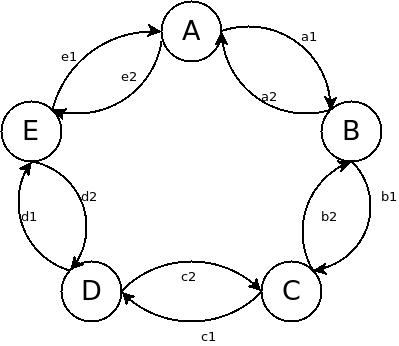
\includegraphics[width=0.5\textwidth]{Imagen/ejercicio5tema3.jpg}
	\caption{Anillo STM-16}
	\end{figure}
	\begin{tabular}{c|c|c|c|c|c|c|c|c|c|c|c|c|c|c|c|c|}
		   & 1  & 2  & 3  & 4  & 5  & 6  & 7  & 8  & 9  & 10 & 11 & 12 & 13 & 14 & 15 & 16 \\\hline
		a1 &    &    &    &    &    &    &    & EB & AD & AD & AD & EC & EC & AC &    &    \\\hline
		a2 &    &    &    &    &    &    &    & BE & DA & DA & DA & CE & CE & CA &    &    \\\hline
		b1 & BC & BC &    &    &    &    &    &    & AD & AD & AD & EC & EC & AC &    &    \\\hline
		b2 & CB & CB &    &    &    &    &    &    & DA & DA & DA & CE & CE & CA &    &    \\\hline
		c1 &    &    &    & CE & CE & CA &    &    & AD & AD & AD & EC & EC & AC &    &    \\\hline
		c2 &    &    &    & EC & CE & AC &    &    & DA & DA & DA & CE & CE & CA &    &    \\\hline
		d1 &    &    &    &    &    &    &    &    &    &    &    &    &    &    &    &    \\\hline
		d2 &    &    &    &    &    &    &    &    &    &    &    &    &    &    &    &    \\\hline
		e1 & DA & DA & DA &    &    & CA &    & EB & AD & AD & AD & EC & EC & AC &    &    \\\hline
		e2 & AD & AD & AD &    &    & AC &    & BE & DA & DA & DA & CE & CE & CA &    &    \\\hline
	\end{tabular}
\end{exercise}
\begin{exercise}[6]
	Decodifique y determine la secuencia de alineamiento del interfaz U de un acceso primario en el que se recibe la siguiente colección de bits sabiendo que los primeros 8 bits del canal número 3 son 00001000: ···-0+0-+-00+-000+-00-00+000-+00-+00+0-000-+-+000+-+-···\\
	Lo primero vemos que al tratarse de un acceso primarioel mensaje está codificado en HDB3. El primer paso para resolver el ejercicio será la decodificación completa. Hay que tener en cuenta que cada vez que se rompa la alternancia de más y menos este el bit que la rompe será un cero. Asimismo, los tres bits anteriores también serán ceros.\\
	Mensaje descodificado: 10101110011000100000010001100100000100001110000111. Después de esto solo queda identificar los primeros 8 bits del canal 3 y de ahí contar 16 bits hacia atrás para encontrar los 8 bits de alineamiento. Se puede ver que existen dos posibles inicios del canal 3. El primero no puede ser, ya que no está suficientemente retrasado para incluir la trama de alineamiento en el mensaje descodificado. El segundo, en cambio si, podemos ver que la trama lleva una alineación como la siguiente: 00110001.
\end{exercise}
\begin{exercise}[7]
	Se desea establecer un enlace RDSI entre dos ciudades que distan 35km e intercambian un tráfico de 102E, con el objetivo de que la probabilidad de pérdida de llamadas de los usuarios sea inferior al 1\%. Los circuitos necesarios se implementarán mediante multiplex MIC de norma europea. Se ha decidido tener una línea de postes con un único cable 25-CEF (25 pares con aislamiento de plástico de calibre 0.91 mm), que se utilizará para la transmisión en BF y MIC, cuyos parámetros a la frecuencia de 1024 kHz son:
\begin{itemize}
	\item Atenuación: $12\sfrac{dB}{km}$
	\item Atenuación de diafonía para una longitud de 1km: 15dB
\end{itemize}
Se estima que el ruido térmico y de intermodulación se pueden despreciar frente a la diafonía y que la atenuación de diafonía en función de la longitud del cable se puede expresar como:
\[A_D(L)=A_D(L_0)+10log(\frac{L}{L_0}\]
Para las secciones de regeneración, se dispone de regeneradores de 42 dB de ganancia, con una sensibilidad a la diafonía de 18 dB. Se reservarán tres pares de cable para supervisión. El departamento de contabilidad de la compañía suministra los siguientes datos (miles de €):
\begin{center}
\begin{tabular}{c c c}
	\hline
	\textbf{Concepto} & \textbf{Mano de obra} & \textbf{Materiales}\\\hline
	Mux digital (mux y demux) & 3 & 5,5\\
	ETL (tx y rx) & 1,5 & 1,8\\
	Tendido de 1km de cable & 0,35 & 0,5\\
	Repetidor intermedio bidireccional & 1 & 0,8\\
	Instalación de 1km de línea de postes & 0,6 & 0,12\\\hline
\end{tabular}
\end{center}
Las secciones de regeneración se dispondrán siguiendo el esquema de la siguiente figura:
\begin{figure}[htp]
\centering
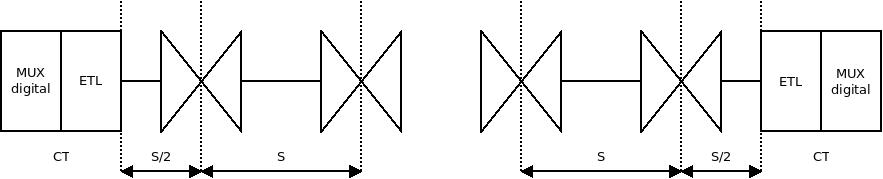
\includegraphics[width=\textwidth]{Imagen/ejercicio7tema3.jpg}
\caption{esquema de las secciones de regenaración}
\end{figure}
Nota: Para el cálculo de la diafonía se puede suponer que las señales del sistema perturbador y del perturbado tienen la misma potencia.\\
Se pide:\\
1. Determine el número de multiplex MIC necesarios\\
2. Determine la longitud máxima de los tramos cuya atenuación puede ser compensada por los regeneradores\\
3. ¿Cuántos pares son susceptibles de ser explotados en BF?\\
4. Determine la longitud de la sección de regeneración\\
5. Inversión inicial\\
holi
\end{exercise}
\begin{exercise}[8]
	En las figuras (a) y (b) se muestran dos esquemáticos de sistemas ópticos, válidos para WDM, se le pide que calcule las pérdidas totales por inserción entre
\begin{enumerate}
	\item Entrada y salida de figura (a)
	\item A y B en el ADM óptico de la figura (b)
	\item A y C en el ADM óptico de la figura (b)
\end{enumerate}
\begin{center}
\begin{tabular}{c c}
	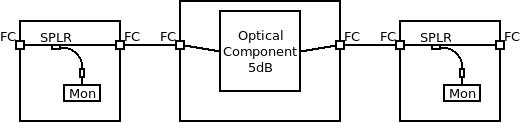
\includegraphics[width=0.4\textwidth]{Imagen/ejercicio8tema3a.jpg}
	& 
	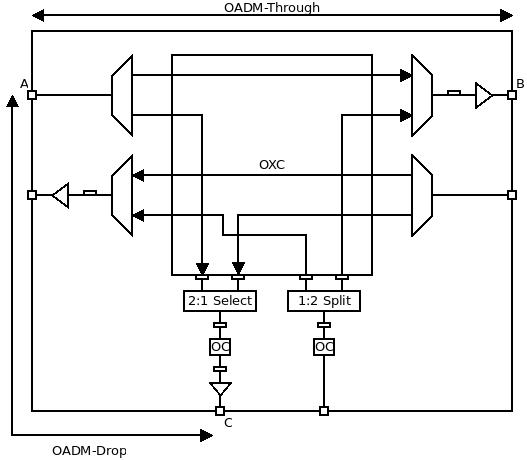
\includegraphics[width=0.4\textwidth]{Imagen/ejercicio8tema3b.jpg} \\
	Figura (a) & Figura (b)
\end{tabular}
\end{center}
Sabiendo que cada dispositivo monitor (Mon) añade 0.6 dB de pérdidas, y el resto de parámetros se muestran en la tabla siguiente:
\begin{center}
\begin{tabular}{c | c}
\hline
	\textbf{Componente} 	& \textbf{Valor}\\\hline
	Fibra Monomodo			& 0,1dB/km\\
	Conector de Fibra		& 0,4dB\\
	Conector Multifibra		& 0,5dB\\
	Empalme (Splice)		& 0,2dB\\
	Mux óptico				& 1dB/canal\\
	Demux óptico			& 1dB/canal\\
	OXC (through)			& 0,5dB\\
	OXC (drop)				& 2dB\\
	Divisor (splitter)		& 3dB\\
	Tap						& 0,2dB\\
	Selector 2:1			& 3dB\\
	Filtro					& 0,5dB\\
	Ganancia Amplificador	& 6dB\\
	Convertidor de $\lambda$ (OC)	& 1dB\\\hline
\end{tabular}
\end{center}
\textbf{1. Entrada y salida de la figura (a)}\\
\[L_{AB}=6FC+2SPLR+5dB+2Mon=14,6dB\] 
\textbf{2. A y B en el ADM óptico de la figura (b)}\\
\[L_{AB}=2FC+1Demux+1OXC(through)+1Mux+1Splice-G_{AO}=-3.5\sfrac{dB}{canal}\]
\textbf{3. A y C en el ADM óptico de la figura (b)}\\
\[L_{AC}=2FC+1Demux+1OXC(Drop)+1Selector+1OC+3Splice-G_{AO}=2,4\sfrac{dB}{canal}\]
\end{exercise}
\begin{exercise}[9]
	Se desea calcular la potencia total recibida en un sistema DWDM en el que hay 40 canales, y que se transmite en una fibra mono-modo que tiene una atenuación de 0.1dB/km, y una dispersión cromática de 0.5ps/nm·km y una dispersión por polarización de 0.12ps/$\sqrt{km}$. El sistema cuenta con 40 canales en la banda C, separados 100nm, y cada uno a 10Gbps. El transmisor, un laser, es capaz de acoplar 0dBm a la fibra con una precisión de f±20nm. Como receptor se tiene un diodo APD, que tiene una sensibilidad de -33dBm para obtener una BER de $10^{-9}$ . Las pérdidas del multiplexor/demultiplexor de paso son 7dB, mientras que las del de extracción son de 8dB. El amplificador tiene una ganancia de 0dB, en cada empalme se pierden 0.2dB y en cada conector 0.5dB. En los 80km de longitud del sistema, hay 4 conectores, 10 empalmes y se espera que en el futuro pueda haber 4 empalmes más. Además, se dejan 2dB de margen para otras degradaciones en el sistema.\\
1. Calcular la potencia recibida\\
2. ¿Permite el sistema margen para futuros empalmes?\\
3. ¿Cumple las especificaciones?
\end{exercise}
\begin{exercise}[10]
	Calcule el span de un sistema en el que se utiliza fibra mono-modo cuya atenuación son 0,1dB/km y su dispersión cromática son 21ps/nm·km con modulación NRZ. El láser es del tipo DFB y es capaz de acoplar a la fibra una potencia de 0dBm. Para compensar la dispersión cromática se utilizan DCF, que no obstante dejan una dispersión residual de 2ps/nm·km añadida. La sensibilidad cromática de estos DCF es de 50ps/nm, y su sensibilidad en recepción es de -1.32 dBm, pero cuentan con una etapa amplificadora de 3dB a su salida. Las pérdidas introducidas por los conectores es de 0,4dB por conector.\\
Nota: Para cada DCF se necesitan dos conectores.
\end{exercise}
%% Tema 4
\section{Redes de comunicaciones moviles terrestres}
\subsection{Sistemas PMR y PMT}
\begin{itemize}
\item{PMR(Private Movil Radio):} Sistemas normalmente no conectados a la red telefónica pública conmutada que se modelan como sistemas de espera.
\item{PMT(Personal Movil Telecommunications):} Sistemas conectados a la red telefónica pública modelados como sistemas con pérdidas. 
\end{itemize}
\subsubsection{Private Movil Radio}
\label{ssub:PMR}
Las características que definen este sistema son las siguientes:
\begin{itemize}
	\item Tienen una area territorial limitada.
	\item No suelen estar conectados a la red telefónica pública conmutada(POTS).
	\item Se suelen usar para dar servicios de empresa como la gestión de flotas.
	\item Deben ser posibles tanto las llamadas entre estaciones moviles (MS) entre sí como las llamadas a grupos.
	\item Deben funcionar en regimen de espera con llamadas frecuentes y de corta duración.
	\item Lo normal es que funcionen en simplex pero hay casos de sistemas en semiduplex e incluso en full-duplex.
\end{itemize}
El ejemplo más representativo de los sistemas PMR es el sistema Trans European Trunked RAdio (TETRA). Dependiendo de como se asignen los canales de comunicación a los ususarios del sistema se puede distinguir entre los dos siguientes sistemas:
\begin{itemize}
	\item Asignación rígida: a un conjunto de ususarios se les asigna un único canal para la comunicación. Es un sistema de asignación bastante poco efectivo, por esto, se suele usar con colectivos relativamente pequeños.
	\item Asignación troncal: se tienen N canales que pueden ser usados por M usuarios.
\end{itemize}
l
\begin{example}[Sistemas PMR]
Se tiene un sistema PMR en el que los usuarios piden 1 llamada de 20 segundos por HC
\begin{gather*}
	\mu=\sfrac{1}{20}s^{-1}\\
	a_o=\frac{\lambda}{\mu}=\frac{20}{3600}=5.56mE	
\end{gather*}
\end{example}
% subsubsection PMR (end)
\subsection{Sistema \acrshort{GSM}}
\label{sub:GSM}
El sistema \acrshort{GSM} tiene está definido por las siguientes características:
\begin{itemize}
	\item Modulación GMSK
	\item Una protección cocanal $\frac{C}{I}=9dB$
	\item Una protección contra dispersión dopler capaz de mantenerse hasta a 200 km/h
	\item Una interferencia base con 6 celdas $i_0=6$
	\item Se trata de un sistema \acrshort{FDD}/\acrshort{FDMA}/\acrshort{TDMA}
	\begin{itemize}
		\item \acrshort{FDD} la subida y bajada se encuentran separadas en diferentes bandas de frecuencia
		\item \acrshort{FDMA}/\acrshort{TDMA} los canales se encuentran en diferentes frecuencias y slots temporales. Con esto un canal viene definido con 2 parámetros, frecuencia y slot temporal.
	\end{itemize}
	\item Cada frecuencia portadora tiene 8 slots temporales o canales.
	\item Este sistema incluye Frecuency Hoping (\acrshort{FH}) con el cual cada trama de la comunicación se transmite en una frecuencia diferente siguiendo un esquema preestablecido.
	\item DTX o transmisión discontinua, solo se transmite información cuando se está hablando, el resto se rellena con ruido blanco para evitar el disconfort al ususario.
\end{itemize}
\subsubsection{Arquitectura del sistema \acrshort{GSM}}
\label{ssub:arquiGSM}
En la imagen se puede ver la arquitectura de red del sistema \acrshort{GSM} con todas sus partes.
\begin{figure}[H]
\centering
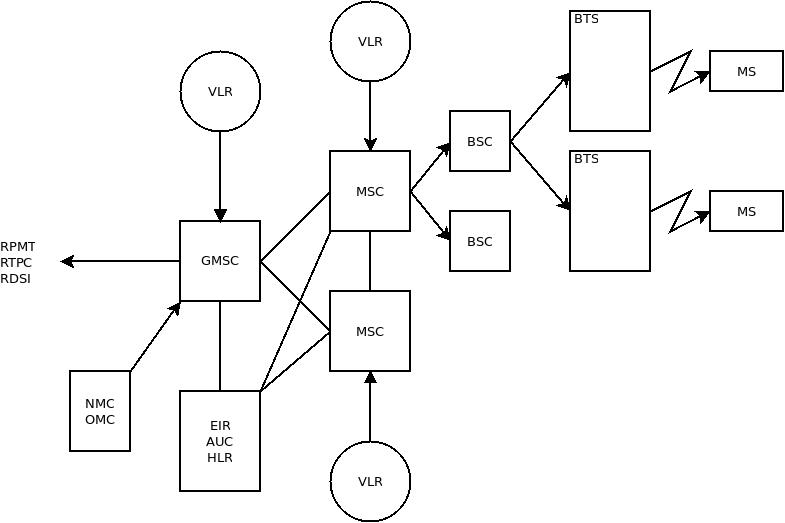
\includegraphics[width=\textwidth]{Imagen/diaGSM.jpg}
\caption{Arquitectura del sistema \acrshort{GSM}}
\label{img:arquiGSM}
\end{figure}
\begin{itemize}
	\item Base Transmission Station (\acrshort{BTS}): Se trata de la antena y los amplificadores de señal, no contiene ningún tipo de "inteligencia", todo se controla desde otros subsistemas.
	\item Mobile Station (\acrshort{MS}): Sistema móvil.
	\item Base Station Controler (\acrshort{BSC}): Controla una o varias \acrshort{BTS} variando potencias transmitidas y canales usados por cada una de ellas.
	\item Mobile Switching Center (\acrshort{MSC}): Controla varias \acrshort{BSC}'s. Están conectadas entre sí en malla.
	\item Gateway Mobile Switching Center (\acrshort{GMSC}): Un \acrshort{MSC} elegido para servir de conexión entre la red móvil y otras redes, como la POTS o Internet. Solo puede haber una por red móvil.
	\item Home Location Register (\acrshort{HLR}): Base de datos de usuarios, contiene la información del \acrshort{MSC} al que se encuentra conectado, datos de tarificación, etc.
	\item Visitor Location Register (\acrshort{VLR}): Cada \acrshort{MSC} tiene uno conectado directamente y se encarga de mantener los datos de usuario de los usuarios conectados a dicho \acrshort{MSC}. Este sistema descarga tráfico del \acrshort{HLR}. Cada vez que un nuevo ususario se registra en el \acrshort{MSC} ha de solicitar su información al \acrshort{HLR}.
	\item Operational Management Center (\acrshort{OMC}): Centro de gestión de características de las \acrshort{BTS}  del sistema.
	\item Network Management Center (\acrshort{NMC}): Centro de gestión de ususarios.
	\item Equipment Identifier Register (\acrshort{EIR}): Base de datos de equipos invalidados, lista negra de moviles robados, basicamente.
	\item Authentication Center: Base de datos con las claves de autenticación de los usuarios del sistema.
	\item Interfaz U: interfaz de conexión radio entre las \acrshort{BTS} y las \acrshort{MS}.
	\item Interfaz de linea o interfaz A: interfaz de conexión entre las \acrshort{MSC} y las \acrshort{BSC}.
	\item Interfaz A-bis: interfaz de conxión entre las \acrshort{BSC} y las \acrshort{BTS}. Esta interfaz surje junto a la idea de conectar varias \acrshort{BTS} a una sola \acrshort{BSC}, en las especifiaciones iniciales esto no era necesario.
\end{itemize}
% subsubsection arquiGSM (end)
\subsubsection{Servicios del sistema \acrshort{GSM}}
\label{ssub:serviciosGSM}
Hay dos servicios básicos. Portadores y teleservicios. Los servicios portadores ofrecen una capacidad de transporte en régimen síncrono/asíncrono en modocircuito o paquete con velocidades hasta 9600bps.Los teleservicios, o servicios ofrecidos por el \acrshort{ISP}, son la telefonía digital a dos velocidades: total a 13kbps o mitad a 6,5kbps, los mensajes cortos y los facsímil, FAX del grupo 3. Algunos ejemplos de servicios suplementarios son, la identificación de llamante, redireccionamiento de llamadas, llamada en espera, buzón de voz, conferencias pluripartitas y la tarificación.
% subsubsection serviciosGSM (end)
\subsubsection{Tramas del sistema \acrshort{GSM}}
\label{ssub:tramaGSM}
Cada trama básica del sistema \acrshort{GSM} está constituida por 8 intervalos de 0,577ms durando la trama 4,615ms en total. Los enlaces descendentes y ascendentes para cada canal están decalados 3 timeslots pudiendo así usarse la misma antena para ambos enlaces. Cada ráfaga está compuesta por 148 bits. estos bits se organizan, como se puede ver en la imagen, de la siguiente forma.
\begin{itemize}
	\item 6 bits de cabecera (Tail Bits).
	\item 116 bits de datos, de los cuales 2 son flags que indican si se trata de un mensaje TCH o \acrshort{FACCH}.
	\item 26 bits de entrenamiento para la estimación del canal y del equalizador.
	\item Un tiempo de guarda equivalente a 8,25 bits. Para la sincronización entre los usuarios.
\end{itemize} 
\begin{figure}[H]
\centering
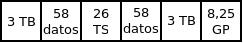
\includegraphics[width=0.6\textwidth]{Imagen/tramaGSM.jpg}
\caption{Estructura de una trama normal de datos de \acrshort{GSM}}
\label{img:tramaGSM}
\end{figure}
Con esta estructura se puede ver que la velocidad de transmisión del enlace radio del sistema \acrshort{GSM} es: $\sfrac{156,25bits}{0,577ms}=270,833kbps$\\
Para reducir la cantidad de señalización necesaria, las tramas se agrupan en multitramas, supertramas e incluso hipertramas. Las supertramas de 26 tramas se usan para los canales de tráfico, las de 51 tramas, en cambio, se usan para canales de señalización y control.
% subsubsection tramaGSM (end)
\subsubsection{Canales del sistema \acrshort{GSM}}
\label{ssub:canalesGSM}
Los canales en \acrshort{GSM} se dividen en canales de tráfico y canales de señalización. Los canales de tráfico siempre vienen definidos por el par de portadoras y timeslots asignados para la comunicación. Se han especificado 7 posibles canales de tráfico:
\begin{itemize}
	\item Voz a velocidad total (TCH/F)
	\item Voz a velocidad mitad (TCH/H)
	\item Datos a velocidad de 2,4, 4,8 y 9,6 kbps
	\item Datos a velocidad mitad de 2,4 y 4,8 kbps
\end{itemize}
Estos canales tienen asociados dos canales de señalización, el \acrshort{SACCH} y el \acrshort{FACCH}. El Slow Associated Control Channel (\acrshort{SACCH}) es el canal que transmite la señalización necesaria para mantener la llamada, como, control de potencia, calidad del canal, tarificación, etc. El Fast Associated Control Channel (\acrshort{FACCH}) es el canal que transmite los mensajes urgentes relacionados con la llamada, como un traspaso de celda. El \acrshort{FACCH} utiliza espacio del canal de información debido al carácter urgente de la información que se transmite en él. A parte hay otros canales de señalización descritos a continuación:
\begin{itemize}
	\item Canales de difusión, canales descendentes que transmiten a todos los terminales móviles informaciones varias.
	\begin{itemize}
		\item Broadcast Control CHannel (\acrshort{BCCH}), transmite información general de la red y la celda para la orientación.
		\item Frecuency Correction CHannel (\acrshort{FCCH}), envía información precisa sobre las portadoras utilizadas por la \acrshort{MS}.
		\item Synchronization CHannel (\acrshort{SCH}), difunde información sobre sincronización de trama e identificación de la \acrshort{BTS}.
	\end{itemize}
	\item Canales comunes (\acrshort{CCH}), se utilizan para regular el acceso al sistema de los terminales. Los hay ascendentes y descendentes.
	\begin{itemize}
		\item Random Acces CHannel (\acrshort{RACH}), canal ascendente usado para la solicitud de recursos al sistema por parte de las \acrshort{MS}. Utiliza el protocolo ALOHA ranurado para controlar el acceso múltiple de las \acrshort{MS} al canal.
		\item Paging CHannel (\acrshort{PCH}), canal descendente por dodne se notifica a las \acrshort{MS}  de una llamada destinada a la misma.
		\item Access Grant CHannel (\acrshort{AGCH}), canal descendente usado para la asignación de canales previamente solicitados por el \acrshort{RACH}.
	\end{itemize}
	\item Los canales dedicados son canales bidireccionales que se asignan a las \acrshort{MS} en exclusiva durante los momentos previos a la llamada.
	\begin{itemize}
		\item Stand-alone Dedicated Control CHannel (SDCCH), se divide en 8 canales vinculados a diferentes \acrshort{MS} para el intercambio de información de señalización.
		\item Slow Associated Control CHannel (\acrshort{SACCH}), es el canal de señalización lenta asociada a la información transmitida por el SDCCH. está dividido en 8 cnanales vinculados a los 8 del SDCCH.
	\end{itemize}
\end{itemize}
% subsubsection canalesGSM (end)
% subsection GSM (end)
\subsection{Universal Mobile Telecommunication System (UMTS)}
\label{sub:UMTS}

% subsection UMTS (end)
\subsection{Long Term Evolution (LTE)}
\label{sub:LTE}
	
% subsection LTE (end)
\subsection{Ejercicios}
\label{sub:ejercicios4}
\begin{exercise}[1]
	Un sistema celular formado por clusters de 4 celdas hexagonales de 1.38 km de radio, dispone de 60 canales. El tráfico ofrecido por cada usuario es de 0.029 E, que corresponden a una llamada en media por HC. Se trata de un sistema dotado de colas de espera, con objetivo de que la probabilidad de que un usuario tenga que esperar sea menor o igual que el 5\%. Se pregunta: \\
	\textbf{1.} ¿Cuántos usuarios por km2 puede soportar el sistema? \\
	Suponiendo celdas unisectoriales, podemos ver que cada celda tendrá asignados $\frac{c}{J}=\frac{60}{4}=15\sfrac{canales}{celda}$ con este dato y la probabilidad de espera, $P_B=0,05$, se puede obtener el tráfico ofrecido a la celda gracias a la función Erlang C. 
	\[C(c,A_o)=0,05\to A_o=8E\]
	Con estos datos y sabiendo que el tráfico por usuario es $a_o=0.029E$ obtenemos:
	\[N_{celda}=\frac{A_o}{a_o}=\frac{8}{0,029}=275\sfrac{usuarios}{celda}\]
	Sabiendo los usuarios por celda y el tamaño de la celda, la densidad de usuarios tendrá que ser menor que D para permanecer dentro de las especificaciones del sistema:
	\[D=\frac{N_{celda}}{S_{celda}}=\frac{275}{4.95km^2}=55,58\sfrac{usuarios}{km^2}\]
	\textbf{2.} ¿Cuál es la probabilidad de que una llamada espere más de 10 segundos?
	\[a_o=\frac{\lambda}{\mu}\to \mu=\frac{\lambda}{a_o}=\frac{1}{0,029}=34,48\sfrac{llamadas}{HC}=0.01\sfrac{llamadas}{s}\]
	\[P(t\geq 10s)=1-e^{-\mu 10}=0,09\]
\end{exercise}
\begin{exercise}[2]
	Un sistema PMR de asignación troncal dispone de las siguientes bandas de frecuencia, dentro de la banda asignada: 380-382/390-392MHz, con canalización de 25kHz. Sobre cada portadora se establece una trama con cuatro intervalos de tiempo, sobre la que se realizará un acceso múltiple TDMA/FDMA. La velocidad binaria en la interfaz radio es de 30 kbps. Con este sistema se pretende prestar un servicio de gestión de flotas a una compañía que opera en el centro de Madrid, constituida por un total de 100 vehículos. Se estima que la gestión de la flota requiere cursar un tráfico de 0.7E en sentido despacho$\to$flota y 0.3E en sentido flota$\to$despacho, ambos en la hora cargada (utilizando canales de 7.5kbps en cada sentido). Se requiere operación full-duplex. Se pregunta:\\
	\textbf{1.} ¿Cuántas portadoras es necesario habilitar para obtener un grado de servicio del 0.1 \%? Elija los valores de frecuencia\\
	%Como la operación ha de ser full-duplex, y hay dos bandas bien diferenciadas, usaremos FDD para la duplexación.
	%\[c=\frac{BW}{BW_{porta}}=\frac{2MHz}{25\sfrac{kHz}{portadora}}=80\text{ portadoras full duplex}\]
	En este problema hay dos soluciones bien diferentes basadas en dos suposiciones: 
	\begin{enumerate}
		\item Si suponemos Que los tráficos del enunciado son por vehículo 
		\item Si en cambio los suponemos tráficos totales
	\end{enumerate}
	Si suponemos lo primero:
	\begin{gather*}
		a_o=0,7+0,3=1E\\
		A_o=N*a_o=100E\\
		GoS=0,001=C(c,A_o)\to c\approx 200canales\\
		\Delta f=c\frac{1}{4\sfrac{canales}{portadora}}25\sfrac{kHz}{portadora}=1,25MHz
	\end{gather*}
	En este caso las bandas utilizadas serían:380-381,25/390-391,25MHz.\\
	Si en cambio suponemos tráficos totales:
	\begin{gather*}
		A_o=0,7+0,3=1E\\
		GoS=0,001=C(c,A_o)\to c\approx 6canales\\
		\Delta f=c\frac{1}{4\sfrac{canales}{portadora}}25\sfrac{kHz}{portadora}=50kHz
	\end{gather*}
	En este caso las bandas utilizadas serían:380-380,05/390-390,05MHz.\\
	\textbf{2.} Obtenga el valor de la eficiencia de trunking (número de usuarios por canal)\\
	Estamos en el mismo problema que antes, hay dos casos.\\
	En el caso de ser tráfico por usuario:
	\[\eta=\frac{N}{c}=\frac{100}{200}=0,5\sfrac{usuarios}{canal}\]
	En el caso de ser tráficos totales:
	\[\eta=\frac{N}{c}=\frac{100}{6}=16,67\sfrac{usuarios}{canal}\]
	\textbf{3.} ¿Qué grado de servicio se obtendría si se utilizara asignación fija con el mismo número de usuarios por canal?
	Estamos en el mismo problema que antes, hay dos casos.\\
	En el caso de ser tráfico por usuario:
	\begin{gather*}
		A_o=a_o \eta=0.5E\\
		GoS=0,5
	\end{gather*}
	Como se puede ver al pasar de trunking a asignación fija el grado de servicio baja al 50\%.\\
	En el caso de ser tráficos totales:
	\begin{gather*}
		a_o=\frac{A_o}{N}=0.01E
		A_o=a_o \eta=0.1667E\\
		GoS=0,1667
	\end{gather*}
	Como se puede ver al pasar de trunking a asignación fija el grado de servicio baja al 16,67\%, no se ve una mejora tan inmensa como en el otro caso, pero sigue siendo considerable.\\
\end{exercise}
% subsection ejercicios4 (end)
%% Tema 5
\section{Sistemas de Radiocomunicación por Satélite}
\label{sec:satelite}
	\subsubsection{Introducción e historia}
	\label{ssub:introSat}
		El objetivo delos sistemas de radiocomunicación por satelite es el establecimiento de enlaces entre estaciones, tanto fijas como móviles, mediante repetidores en la órbita terrestre. Este concepto se refleja ya en artículos desde 1929. Los repetidores pueden ser tanto activos como pasivos, es decir, pueden amplificar la señal o no.\\
		La carrera espacial empieza con la idea de utilizar el espacio para lo militar. En 1957 se lanzan los primeros Sputnik y a Laika. Mientras tanto en estados unidos crean la NASA, sin lanzar nada al espacio. A partir de 1958 se empiezan a lanzar satelites de comunicación de la NASA con el departamento de defensa yanki. El primero fue un repetidor pasivo. En 1963 se pone en orbita el primer satélite geoestacionario, el Syncom 2.\\
		En 1964 se crea INTELSAT, una organización de 11 paises para la creación de un sistema comercial mundial de telecomunicaciones vía satélite. En la actualidad es privado y lo componen 109 paises. El primer satélite fue el early bird (INTELSAT I).\\
		Los sistemas satélite son una alternativa a otros sistemas. Con 3 satélites geoestacionarios se puede cubrir toda la superficie terrestre. Los equipos de comunicación y control deben ser muy fiables, ya que, la reparación puede ser imposible, además de estar expuestos a gran cantidad de radiaciones. Tienen una vida util limitada por el fin del combustible usado para los motores, una vez sin combustible no se pueden reorientar y se envian a una órbita basura. Los sistemas satélite se suelen usar como complemento, por ejemplo, un cable submarino puede tener un sistema satélite de soporte.
	% subsubsection introSat (end)
	\subsubsection{Servicios de satélites}
	\label{ssub:serviciosSat}
		\begin{itemize}
			\item Servicio fijo: Enlaces entre dos puntos terrestres usando el satélite como repetidor.
			\item Servicio Móvil: Uno o más puntos fijos y móviles, como barcos, aviones y torres de control.
			\item Servicio de radiodifusión: Uno o más puntos fijos y terminales dispersos, como la televisión o la radio satélite.
			\item Servicio de radiodeterminación: Localización determinada por satélites, como los sistemas GPS o Galileo.
			\item Servicio de exploración de la tierra: desde mapas del tiempo (meteosat), creación de mapas hasta la exploración de recursos.
			\item Servicio de exploración del espacio: mediante el uso de telescopios o radiotelescopios como el Hubble.
			\item Servicio entre satélites: La comunicación entre satélites no tiene limitaciones físicas para el uso de ancho de banda, por ejemplo, a 60GHz el oxígeno absorbe la señal, en el espacio no.
		\end{itemize}
	% subsubsection serviciosSat (end)
	\subsubsection{Estructura del sistema de comunicación satélite}
	\label{ssub:estructSat}
		\begin{figure}[htp]
			\centering
			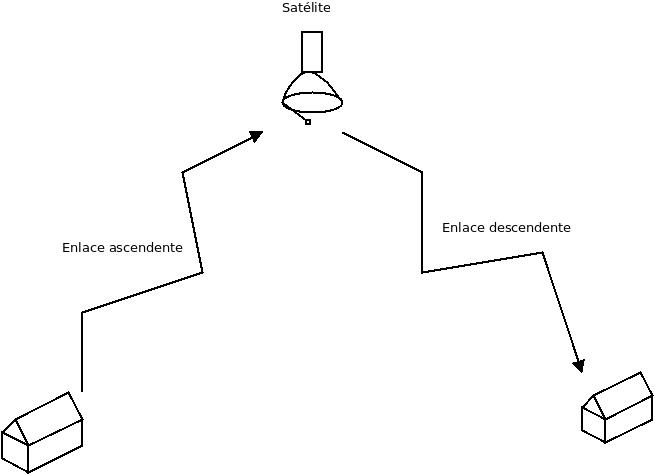
\includegraphics[width=0.7\textwidth]{Imagen/arquisatelite.jpg}
			\caption{Estructura de un sistema de comunicación satélite}
		\end{figure}
		\begin{itemize}
			\item Estación terrena de transmisión: Recibe la señal para posteriormente modularla a una radiofrecuencia (RF), amplificarla y después transmitirla. En transmisión se necesita mucha potencia y una gran directividad.
			\item Enlaces: tanto el enlace ascendente como el descendente se modelan como sistemas de transmisión en espacio libre con pérdidas ocasionadas por la frecuencia, distancia, atmosfera e incluso la lluvia.
			\item Satélite: Se trata de una estación repetidora, que amplifica, cambia de banda y retransmite las señales. Las partes involucradas en cada acción vienen descritas a continuación:
			\begin{itemize}
				\item Recepción: La antena, un filtro y un amplificador de bajo ruido.
				\item Transpondedor: Se trata de un conversor de frecuencia y amplificador encargado de llevar a cabo la retransmisión.
				\item Conmutación: piezas encargadas del encaminamiento y por tanto de la asignación de transpondedores.
				\item Transmisión: Amplificación, filtrado y antena de transmisión.
			\end{itemize}
			\item Estación terrena de recepción: Hace uso de un recptor superheterodino, receptor de ondas de radio que utiliza un proceso de mezcla de frecuencias o heterodinación para convertir la señal recibida en una a frecuencia intermedia. Esta señal sin la radioportadora de alta frecuencia es mucho más facil de manejar que la original.
			\item Segmento espacial: La suma de los retardos en los enlaces, en transmisión, en recepción y en el satélites terminan produciendo grandes retardos, 250ms en geoestacionarios. Este hecho hace necesario el uso de técnicas de cancelación de ecos.
		\end{itemize}
		El diseño de estos sistemas de comunicación satélite tiene que tener en cuenta los siguientes aspectos:
		\begin{itemize}
			\item Órbita: En la mayoría de las ocasiones se utiliza una órbita geoestacionaria. Para comunicaciones móviles se empiezan a utilizar órbitas meo y leo para reducir el retardo y la potencia transmitida.
			\item Cobertura: Se pueden usar varios transpondedores para poder conformar un haz de diferente tipo y anchura.
			\item Conectividad: Capacidad de establecer enlaces entre estaciones terrenas. 
			\item Técnicas de acceso múltiple para la compartición del satélite. Se suelen utilizar FDMA y TDMA, en algunas ocasiones se puede utilizar CDMA pero supone un gran problema.
			\item Banda de frecuencia y ancho de banda: Se utilizan diferentes bandas según el servicio y la disponibilidad necesitada. Las bandas a mayor frecuencia han de transmitir más potencia para superar la peor propagación. Para aumentar la reutilización se separan haces de la misma frecuencia polarizandolos opuestos. Para aumentar aún más la eficiencia se mejoran el tratamiento de la señal y las modulaciones.
			\item Potencia: Se busca un compromiso entre la distancia a recorrer y la limitación a bordo del satélite. Una nueva limitación es la interferencia con otros satélites y estaciones terrenas.
		\end{itemize}
	% subsubsection estructSat (end)
	\subsubsection{Órbitas}
	\label{ssub:orbitas}
		Las óbitas se basan en las leyes de Kepler, consecuencia de la ley de gravitación universal. La elección de la órbita depende del tipo de cobertura, aplicación o recursos económicos. Las órbitas disponibles son escasas. Existen dos tipos de órbitas, las geoestacionarias y las oblícuas. Las órbitras geoestacionarias (GEO) son órbitas circulares, en una latitud baja, inclinación nula y un periodo de revolución igual al ciclo terrestre. Estos satélites siempre son visibles y no requieren, teoricamente, de un seguimiento. En las órbitas oblicuas, en cambio, el seguimiento ha de ser continuo, ya que el satélite sale y se pone. Dependiendo de la altura de la órbita puede ser: baja (LEO), media (MEO) o alta (HEO). Tanto los LEO como los MEO son más baratos de lanzar que los GEO.\\
		Las ventajas de las órbitas de tipo geoestacionaria son, la gran superficie de cobertura y permiten la existencia de estaciones terrenas fijas. Las mayores desventajas son la potencia necesaria para la transmisión, las antenas necesarias, los retardos, los lanzamientos de alto coste y la imposibilidad que presentan de cubrir latitudes altas.
		La órbita geoestacionaria viene definida por la siguiente formula, tomando los siguientes valores. $\omega=\frac{2\pi}{T}$ para un periodo de rotación T=23h 56min.
		\[G\frac{Mm}{d^2}=md\omega^2\]
		De esta formula y teniendo en cuenta un radio de la tierra de 6366km, se obtiene una distancia a la superficie de la tierra de 35806km.\\
		La cobertura del satélite tiene dos formas, la cobertura geométrica es la cobertura real que ofrece el satélite, esta es diferente de la cobertura radioeléctrica. La cobertura radioélectrica es igual a la geométrica pero tiene en cuenta el ruido terrestre y los obstáculos físicos, es decir es una cobertura real.
	% subsubsection orbitas (end)
	\subsubsection{Distancias satelitales}
	\label{ssub:distSatelite}
		Las coordenadas cartesianas del satélite son las siguientes: 
		\begin{gather*}
			x_s=R+h\\
			y_s=0\\
			z_s=0
		\end{gather*}
		Las coordenadas de la estación terrena, en cambio:
		\begin{gather*}
			x_e=Rcos\phi cos\lambda\\
			y_e=Rsin\phi cos\lambda\\
			z_e=Rsin\lambda
		\end{gather*}
		Los ángulos $\phi$ y $\lambda$ son longitud y latitud. $\phi$ se calcula como la diferencia entre la longitud del satélite y la longitud de la estación terrena. $\phi_l=\phi_s-\phi_e$. El ángulo $\lambda$ es la latitud de la estación terrena, ya que, la latitud del satélite, al estar sobre el ecuador es 0.\\
		La distancia entre el satélite y la estación terrena se puede calcular por medio de una simple regla de pitagoras:
		\[ES=d=\sqrt{(x_s-x_e)^2+y_e^2+z_e^2}=\sqrt{(R+h)^2+R^2-2R(R+h)cos\phi cos\lambda}\]
	% subsubsection distSatelite (end)
	\subsubsection{Balance de Enlace}
	\label{ssub:balance}
		Es el calculo de potencias que permite determinar la calidad de un enlace. El balance del enlace se puede generalizar con la siguiente formula.
		\[\frac{c}{N_0}=P_{tx}+G_{tx}+\frac{G_{rx}}{T}-L-BO-10logKB\]
		De la fórmula sabemos que T es la temperatura del receptor, K es la constante de Boltzman, B el ancho de banda del canal, L son las pérdidas del enlace, BO es el Back-Off. El back-Off se diferencia en: Input Back-Off para el sentido ascendente y Output Back-Off para el descendente, IBO y OBO. El factor de calidad del enlace es el cociente entre la ganancia y temperatura del receptor.\\
		La calidad del enlace para enlaces digitales se calcula de la siguiente forma:
		\[\frac{e_b}{n_0}=\frac{c}{n_0}\frac{1}{R_b}\]
	% subsubsection balance (end)
% section satelite (end)
\subsection{Ejercicios}
\label{sub:ejercicios5}
\begin{exercise}[1]
	La organización internacional INMARSAT propone diferentes estándares para ofrecer varios servicios marítimos de telecomunicación en banda L. El estándar A reúne las siguientes características:
	\begin{itemize}
		\item Satélite:
		\begin{itemize}
			\item Ganancia en el borde: 16dBi
			\item Potencia transmitida: 10W en un ancho de banda de 2MHz (40 canales)
			\item Temperatura de ruido del sistema: 500K
		\end{itemize}
		\item Estación marítima:
		\begin{itemize}
			\item Potencia transmitida: 10W
			\item Antena de 2m de diámetro y 50\% de eficiencia
			\item Relación G/T: -4$\sfrac{dB}{K}$
		\end{itemize}
		\item Enlaces:
		\begin{itemize}
			\item Estación costera: 4-6GHz
			\item Estación marítima:1.5-1.6GHz
		\end{itemize}
	\end{itemize} 
	DATOS: En la modulación FM, tenemos que $(\frac{S}{N})$,es la relación señal a ruido de la señal demodulada. Donde $p$ y $w$ son factores de ponderación débil en sistemas FM (las bandas altas sufren mayor atenuación). $\Delta_{eff}$ es la excursión efectiva de la señal y $f_m$ es la frecuencia base de la FM. $p+w=7.7dB$. Considere la banda base de la voz como frecuencia base, es decir $f_m=3400Hz$. Recuerde que $\Delta_{eff}=\frac{\delta_{fc}}{\sqrt{2}}$, y que $B_M=2(f_m+\Delta_{fc})$.\\
	\textbf{1.} Obtenga la relación señal a ruido de la señal de voz demodulada en ambos enlaces. Suponga una distancia entre el satélite y la estación marítima de 38000 km.
\end{exercise}
\begin{exercise}[2]
	Se desea diseñar una red VSAT bidereccional en estrella, apoyada en el satélite Hispasat (30 O), con funcionamiento en banda Ku. Tanto el Hub como las estaciones VSAT se encuentran en Madrid (40.5 N, 3.5 O).\\
	Los anchos de banda de RF necesarios son 200kHz para el outbound y 50kHz para el inbound.\\
	El enlace ascendente del Outbound se realiza a 14100MHz, mientras que el enlace descendente tiene lugar a 11800MHz. En el inbound, la frecuencia para el enlace ascendente es de 14300MHz y para el descendente 12000MHz. El satélite tiene una PIRE de 44dBW en un ancho de banda de 72MHz y una $\frac{G}{T}$ de 0$\sfrac{dB}{K}$. Tanto para el inbound como el outbound se utiliza la modulación QPSK. La tasa binaria es de 128kbps para el outbound mientras que es de 32kbps para inbound.
	\begin{itemize}
		\item Los parametros del HUB son:
		\begin{itemize}
			\item Potencia transmitida: 27dBW 
			\item Pérdidas en los terminales: 2dB tanto en transmisión como en recepción
			\item Antenas de 5m de diámetro y 70\% de eficiencia
			\item Temperatura de ruido del sistema: 200K (después de las pérdidas en los terminales)
		\end{itemize}
		\item Los parámetros de las estaciones VSAT son:
		\begin{itemize}
			\item Potencia transmitida: 1W
			\item Antena de 1m de diámetro y 65\% de eficiencia
			\item Pérdidas en los terminales: 1dB tanto en transmisión como en recepción
			\item Temperatura de ruido del sistema: 200K (después de las pérdidas en los terminales)
		\end{itemize}
	\end{itemize}
	DATOS: Radio de la tierra: 6366km. Altura del satélite Hispasat: 35876km. En una QPSK, la probabilidad de error se calcula como $BER=Q(\sqrt{\frac{2e_b}{n_0}})$.\\
	Se pide lo siguiente:\\
	\textbf{1.} Para el enlace Outbound, determine la relación $\sfrac{C}{N}$ en el uplink y downlink\\ 
	\textbf{2.} Determine la relación $\sfrac{E_b}{N_0}$ en el enlace Outbound y la probabilidad de error de bit que se obtiene \\
	\textbf{3.} Repita los apartados anteriores para el enlace inbound
\end{exercise}
\begin{exercise}[3]
	En un cierto sistema, un satélite GPS está situado en un punto P cuyas coordenadas cartesianas respecto de un sistema de referencia con origen en el centro de la Tierra son: $x_p=14913km;y_p=15000km;z_p=21298km$. Sabiendo que las pseudodistancias a dicho satélite medidas por una estación de control situada sobre el eje Y del sistema son: $R_{m1}=27566,59km$ con $f_1=1600MHz$ y $R_{m2}=27703,48km$ con $f_2=1200MHz$. Se pide:\\
	\textbf{1.} Coordenadas de la estación de control \\
	\textbf{2.} Pseudodistancias a la frecuencia $f_1$ por un receptor cuyas coordenadas son $x_r=6375km;y_r=5380km;z_r=6370km$, si el receptor tiene una deriva de 1$\mu$s
\end{exercise}
\begin{exercise}[4]
	El sistema IRIDIUM proporciona servicios de telecomunicación a móviles mediante una constelación de 66 satélites distribuidos en 6 planos a 780km de altura. El ángulo mínimo de elevación es de 8.2º. Se garantiza un retardo mínimo de 2.6 ms y un retardo máximo de 8.22ms en cada sentido de la comunicación entre el móvil y el satélite. Las frecuencias utilizadas para los enlaces móvil-satélite son 1616-1626.5MHz tanto en el UL como en el DL. El sistema de acceso múltiple empleado es un esquema FDMA/TDMA/TDD, de forma que el ancho de banda de cada canal es de 1.2 kHz.\\
	Se desea estudiar un servicio de transmisión de datos a 2.4kbps con modulación QPSK, considerando el valor medio de la elevación entre el mínimo y el máximo especificados. La PIRE del satélite por canal de datos es de -10 DBW, y el factor de mérito de los receptores es de -20dB/K.\\
	\textbf{1.} Determine si se cumple la especificación de retardo máximo\\
	\textbf{2.} Determine el número mínimo de satélites necesarios para garantizar el funcionamiento con el ángulo de elevación mínimo\\
	\textbf{3.} Determine la distancia y el retardo entre un móvil y el satélite para el valor de elevación bajo estudio\\
	\textbf{4.} Calcule la relaciónn portadora a ruido en el enlace descendente satélite-móvil para un único canal\\
	\textbf{5.} Calcule la probabilidad de error de bit en el receptor del móvil
\end{exercise}
\begin{exercise}[5]
	En una red VSAT ofrecida por el satélite HISPASAT 1D (30ºO) y 35685km de altura, el HUB está compuesto por un equipo que es capaz de dar servicio a 10 terminales VSAT y un amplificador de potencia cuya PIRE es de 20dBW y con un ancho de banda de 6MHz. La antena tiene unas dimensiones de 6 m de diámetro y una eficiencia del 85\%. La temperatura de ruido es de 250K.\\
	El transpondedor utilizado para ofrecer el servicio por parte del satélite tiene un ancho de banda de 36MHz, una PIRE de 30dBW en toda la banda, un back-off de entrada de 3dB y uno de salida de 2dB. La antena utilizada es de 5 metros de diámetro, y una eficiencia del 95\%. La temperatura se puede considerar igual que la del HUB.\\
	Por último, los terminales VSAT transmiten una potencia de 5 W utilizando una antena de 2 metros de diámetro y una eficiencia del 70\%. Como son terminales baratos, tienen unas pérdidas adicionales en recepción de 1dB y en transmisión de 2dB. La temperatura se puede asumir que es la misma que el HUB.\\
	NOTA: Utilize 3 decimales de precisión. Para la modulación QPSK se puede asumir una eficiencia de 2bps/Hz y que la $BER=Q(\sqrt{\frac{2e_b}{n_0}})$. El radio equivalente de la tierra es de 6366 km.
	La tasa binaria de las estaciones VSAT es de 400kbps bidireccionales. La modulación utilizada es QPSK tanto en el inbound como en el outbound. Las frecuencias son las siguientes: 1.5/13GHz para comunicación HUB-Satélite y 1.6/12GHz para satélite-VSAT. El sistema utiliza TDM/TDMA.\\
	Se le pide que conteste razonadamente a las siguientes cuestiones referidas al outbound de una estación situada a 20º de longitud este con respecto al HUB, que está situado a 40.2ºN y 3.5ºO: 
	\textbf{1.} La relación portadora a ruido\\
	\textbf{2.} Calcule la probabilidad de error\\
	\textbf{3.} ¿Cuál será la probabilidad de esperar a transmitir un paquete si la tasa total física del transpondedor del satélite que se utiliza es de 1.6Mbps y el tráfico que genera cada VSAT es de 0.25E? 
\end{exercise}
% subsection ejercicios5 (end)
%\printglossary[type=\acronymtype]

\end{document}
